%                                     MMMMMMMMM                                         
%                                                                             
%  MMO    MM   MMMMMM  MMMMMMM   MM    MMMMMMMM   MMD   MM  MMMMMMM MMMMMMM   
%  MMM   MMM   MM        MM     ?MMM              MMM$  MM  MM         MM     
%  MMMM 7MMM   MM        MM     MM8M    MMMMMMM   MMMMD MM  MM         MM     
%  MM MMMMMM   MMMMMM    MM    MM  MM             MM MMDMM  MMMMMM     MM     
%  MM  MM MM   MM        MM    MMMMMM             MM  MMMM  MM         MM     
%  MM     MM   MMMMMM    MM   MM    MM            MM   MMM  MMMMMMM    MM
%
%
%            - META-NET Language Whitepaper | German paper -

\documentclass[]{../../metanetpaper}

\usepackage{booktabs}
\usepackage{longtable}
\usepackage{tabulary}
\usepackage{tabularx}
\usepackage{rotating}
\usepackage{makecell}
\usepackage{multirow}
\usepackage{colortbl}
\usepackage{polyglossia}
\setotherlanguages{german, english}

%!TEX TS-program = xelatex
\RequireXeTeX %Force XeTeX check

\title{Deutsch im Digitalen Zeitalter --- The German Language in the Digital Age}

\subtitle{White Paper Series --- Weißbuch-Serie}

\author{
  Aljoscha Burchardt \\
  Markus Egg \\
  Kathrin Eichler \\
  Brigitte Krenn \\
  Jörn Kreutel \\
  Annette Leßmöllmann \\
  Georg Rehm \\
  Manfred Stede \\
  Hans Uszkoreit \\
  Martin Volk 
}
\authoraffiliation{
  Aljoscha Burchardt~ {\small DFKI}\\
  Markus Egg~ {\small Humboldt-Universität zu Berlin}\\
  Kathrin Eichler~ {\small DFKI} \\
  Brigitte Krenn~ {\small ÖFAI}\\
  Jörn Kreutel~ {\small FH Brandenburg}\\
  Annette Leßmöllmann~ {\small Hochschule Darmstadt}\\
  Georg Rehm~ {\small DFKI} \\
  Manfred Stede~ {\small Universität Potsdam}\\
  Hans Uszkoreit~ {\small Universität des Saarlandes, DFKI} \\
  Martin Volk~ {\small Universität Zürich}
}

\begin{document}

\renewcommand*{\figureformat}{\sffamily\thefigure\autodot}

\maketitle
  
%                                     MMMMMMMMM                                         
%                                                                             
%  MMO    MM   MMMMMM  MMMMMMM   MM    MMMMMMMM   MMD   MM  MMMMMMM MMMMMMM   
%  MMM   MMM   MM        MM     ?MMM              MMM$  MM  MM         MM     
%  MMMM 7MMM   MM        MM     MM8M    MMMMMMM   MMMMD MM  MM         MM     
%  MM MMMMMM   MMMMMM    MM    MM  MM             MM MMDMM  MMMMMM     MM     
%  MM  MM MM   MM        MM    MMMMMM             MM  MMMM  MM         MM     
%  MM     MM   MMMMMM    MM   MM    MM            MM   MMM  MMMMMMM    MM
%
%
%        - META-NET Language Whitepaper | German mocktitle -


\null
\vfill

\pagestyle{empty} 

{\small
  Die Ausarbeitung dieses Weißbuchs wurde mit Mitteln aus dem Siebten Rahmenprogramm und dem Programm zur Unter-stützung der Politik für Informations- und Kommunikationstechnologien der Europäischen Kommission im Rahmen der Verträge T4ME (Finanzhilfevereinbarung 249119), CESAR (Finanzhilfevereinbarung 271022), METANET4U (Finanzhilfevereinbarung 270893) und META-NORD (Finanzhilfevereinbarung 270899) finanziert.\\

  The development of this white paper has been funded by the Seventh Framework Programme and the ICT Policy Support Programme of the European Commission under contracts T4ME (Grant Agreement 249119), CESAR (Grant Agreement 271022), METANET4U (Grant Agreement 270893) and META-NORD (Grant Agreement 270899).
}

\clearpage


\pagenumbering{Roman} 
\setcounter{page}{5}
\pagestyle{scrheadings}


% --------------------------------------------------------------------------
\ssection*{Vorwort}

Dieses Weißbuch gehört zu einer Serie, die Wissen über Sprachtechnologie und deren Potenzial vermitteln soll, und sich insbesondere an Journalisten, Politiker, Sprachgemeinschaften und Lehrende richtet.

Die derzeitige Verfügbarkeit und Nutzung von Sprachtechnologie in Europa variiert stark je nach Sprache. Folglich müssen auch die notwendigen Maßnahmen für die weitere Unterstützung von Forschung und Entwicklung in diesem Bereich variieren. Die Maßnahmen hängen von zahlreichen Faktoren ab, z.\,B.~der Komplexität einer Sprache und der Anzahl ihrer Sprecher.

META-NET, ein von der Europäischen Kommission gefördertes Exzellenznetzwerk, hat die aktuellen Sprachressourcen und -technologien in der vorliegenden Weiß\-buch-Serie analysiert (siehe S.~\pageref{whitepaperseries}). Die Analyse umfasst die 23 europäischen Amtssprachen sowie weitere wichtige nationale und regionale Sprachen Europas. Die Ergebnisse zeigen, dass es bei allen Sprachen beträchtliche Defizite in der technologischen Unterstützung und signifikante Forschungslücken gibt. Die vorliegende ausführliche Expertenanalyse und Bewertung der aktuellen Situation dient dazu, die Wirksamkeit weiterer Forschungstätigkeit zu maximieren.

META-NET besteht aus 54 Forschungszentren aus 33 Ländern (Stand: November 2011, siehe S.~\pageref{metanetmembers}), die mit Interessensvertretern aus Wirtschaft (Softwareunternehmen, Technologieanbietern, Nutzer), Verwaltung, NGOs, Sprachgemeinschaften und europäischen Universitäten zusammenarbeiten. META-NET entwickelt gemeinsam mit diesen Gruppen eine übergreifende Technologievision und eine strategische Forschungsagenda für das mehrsprachige Europa 2020.


% --------------------------------------------------------------------------
\cleardoublepage

\tableofcontents
%\addtocontents{toc}{\protect\thispagestyle{empty}}

\cleardoublepage

\setcounter{page}{1}
\pagenumbering{arabic} 
\pagestyle{scrheadings}


% --------------------------------------------------------------------------
\ssection{Zusammenfassung}

Europa ist in den vergangenen 60 Jahren eine politisch-wirtschaftliche Einheit geworden. Kulturell und sprachlich ist der europäische Raum reich und vielfältig. Von Portugiesisch bis Polnisch, von Italienisch bis Isländisch -- im kommunikativen Miteinander stoßen Europas Bürger, die europäische Wirtschaft und auch die Politik schnell an sprachliche Grenzen. Die Institutionen der EU geben jährlich rund eine Milliarde Euro für die Übersetzung von Texten und das Dolmetschen gesprochener Kommunikation aus, um am Grundsatz der Mehrsprachigkeit festzuhalten. Ist dieser Aufwand tatsächlich notwendig? Moderne Sprachtechnologie und Sprachforschung können einen wichtigen Beitrag leisten, um die Sprachgrenzen zu überwinden. Wenn Europäer sich miteinander unterhalten oder Verträge schließen wollen, kann moderne Sprachtechnologie in Verbindung mit intelligenten Endgeräten und Anwendungen ihnen hierbei künftig helfen -- selbst wenn sie keine gemeinsame Sprache sprechen. 

\boxtext{Sprachtechnologie baut Brücken für Europas Zukunft}

Die deutsche Wirtschaft profitiert überdurchschnittlich vom europäischen Binnenmarkt: 2010 gingen 60,3\% der deutschen Ausfuhren in die EU, weitere 10,8\% in andere europäische Länder. Doch die Geschäftstätigkeit stößt überall dort auf Schwierigkeiten, wo Sprachbarrieren dem Handel massiv im Wege stehen. Insbesondere kleine und mittelständische Unternehmen stehen vor einem mit vertretbarem Aufwand kaum lösbaren Problem. Die einzige (undenkbare) Alternative zum multilingualen Europa würde so aussehen, dass eine einzige Sprache die Vormachtstellung einnimmt und alle anderen Sprachen ersetzt. 

Eine Möglichkeit, Sprachbarrieren zu überwinden, ist das Erlernen von Fremdsprachen. Ohne technologische Unterstützung stellen die 23 Amts\-sprachen der Mitgliedstaaten der Europäischen Union und die rund 60 weiteren Sprachen Europas für die europäischen Bürger und ihre Wirtschaft, für politische Debatten sowie für den wissenschaftlichen Fortschritt jedoch ein unüberwindliches Hindernis dar. 

Die Lösung ist die Entwicklung von Schlüsseltechnologien: Sprachtechnologien bieten den europäischen Akteuren ungeheure Vorteile, nicht nur auf dem gemeinsamen europäischen Markt, sondern auch bei Handelsbeziehungen mit Dritt-, insbesondere Schwellenländern. Sprachtechnologielösungen werden letztendlich als einzigartige Brücke zwischen den Sprachen Europas dienen. Eine unverzichtbare Basis für die Entwicklung dieser Technologien ist eine systematische Analyse der linguistischen Besonderheiten aller europäischen Sprachen. Außerdem muss der derzeitige Stand der Unterstützung durch Sprachtechnologie analysiert werden. 

\boxtext{Sprachtechnologie als Schlüssel für die Zukunft} 
Die derzeit auf dem Markt erhältlichen Tools zur automatischen Übersetzung und Verarbeitung gesprochener Sprache werden den angestrebten Zielen nicht gerecht. Die dominanten Akteure sind privatwirtschaftliche Unternehmen mit Sitz in den Vereinigten Staaten. Bereits Ende der 1970er-Jahre erkannte die EU die tiefgreifende Bedeutung der Sprachtechnologie als Motor für die europäische Einheit und begann ihre ersten Forschungsprojekte zu finanzieren, beispielsweise EUROTRA. Gleichzeitig wurden nationale Projekte ins Leben gerufen. Diese lieferten zwar wertvolle Ergebnisse, führten aber niemals zu einer konzertierten europäischen Initiative. Im Gegensatz zu dieser hochgradig selektiven Förderung haben andere mehrsprachige Gesellschaften wie Indien (22 Amtssprachen) und Südafrika (11 Amtssprachen) langfristige nationale Programme für Sprachforschung und Technologieentwicklung aufgelegt. 

Die heute marktdominanten Sprach\-tech\-no\-logie-Ak\-teu\-re setzen auf ungenaue statistische Ansätze, bei denen keine tiefgreifende linguistische Analysen und Methoden zum Einsatz kommen. So werden Sätze automatisch übersetzt, indem ein neuer Satz mit Tausenden bereits früher vom Menschen übersetzter Sätze verglichen wird. Die Qualität des ausgegebenen Ergebnisses hängt vor allem vom Umfang und der Qualität der verfügbaren Daten ab. Bei der automatischen Übersetzung einfacher Sätze zwischen Sprachen mit ausreichendem Textmaterial kann man nützliche Ergebnisse erzielen. Doch die flachen, statistischen Verfahren sind zum Scheitern verurteilt bei Sprachen mit einem wesentlich geringeren Anteil an Referenzmaterial oder bei Sätzen von komplexer, nichtrepetitiver Struktur. Wenn wir Anwendungen schaffen möchten, die bei sämtlichen europäischen Sprachen ausgezeichnete Leistung bringen, ist eine Analyse der tieferliegenden strukturellen Eigenschaften der Sprachen die einzige erfolgversprechende Methode.

Aus diesem Grund fördert die Europäische Union Projekte wie EuroMatrix und EuroMatrixPlus (seit 2006) oder iTranslate4 (seit 2010). Hier werden durch Grundlagenforschung und angewandte Forschung Ressourcen für hochwertige Sprachtechnologielösungen für alle europäischen Sprachen bereitgestellt. Die europäische Forschung kann bereits zahlreiche Erfolge verbuchen. So nutzen die Übersetzungsdienstleister der Europäischen Union heute die Open-Source-Über\-set\-zungs\-soft\-ware Moses, die überwiegend im Rahmen europäischer Forschungsprojekte entwickelt wurde. Das vom deutschen Bundesministerium für Bildung und Forschung (BMBF) zwischen 1993 und 2000 geförderte Projekt Verbmobil katapultierte Deutschland in der Forschung im Bereich der Übersetzung gesprochener Sprache für einige Zeit in die internationale Führungsposition. Viele der zu dieser Zeit in Deutschland angesiedelten Forschungs- und Entwicklungslabore (z.\,B.~IBM und Philips) sind jedoch mittlerweile geschlossen oder umgezogen. Statt auf den Ergebnissen seiner Forschungsprojekte aufzubauen, hat Europa weiterhin eher isolierte Forschungsaktivitäten verfolgt, die auf dem Markt wenig wirkungsvoll waren. Der ökonomische Wert selbst der frühen Leistungen lässt sich an der Anzahl der Geschäftsausgliederungen erkennen. Ein Unternehmen wie das bereits 1984 gegründete Trados wurde z.\,B.~2005 an SDL mit Firmensitz in Großbritannien verkauft.

\boxtext{Sprachtechnologie trägt zur Einheit Europas bei}
Die bisher erlangten Erkenntnisse legen nahe, dass die heutige hybride Sprachtechnologie, die tiefe Verarbeitung mit statistischen Methoden kombiniert, die Kluft zwischen allen europäischen Sprachen überbrücken kann. Wie diese Weißbuch-Serie zeigt, bestehen jedoch im Hinblick auf die Einsatzfähigkeit von Sprachlösungen und den Stand der Forschung in den verschiedenen europäischen Mitgliedstaaten enorme Unterschiede. Auch wenn Deutschland zu den größeren EU-Sprachen gehört, ist dennoch weitergehende Forschung notwendig, um wirklich effektive Sprachtechnologielösungen für den alltäglichen Einsatz zu verwirklichen. Gleichzeitig stehen die Chancen gut, dass der deutschsprachige Teil Europas in diesem wichtigen Technologiebereich wieder eine international führende Position einnimmt. 

Die Vision von META-NET ist hochqualitative Sprachtechnologie für alle Sprachen Europas, die die politische und wirtschaftliche Einheit in kultureller Vielfalt vollendet. Mithilfe dieser Technologie können bestehende Schranken eingerissen und Brücken zwischen den Sprachen Europas gebaut werden. Hierfür müssen alle Interessengruppen aus Politik, Forschung, Wirtschaft und Gesellschaft ihre Kräfte bündeln.

Diese Weißbuch-Serie flankiert die anderen strategischen Aktivitäten von META-NET. Einen Überblick hierzu finden Sie im Anhang. Aktuelle Informationen, die neueste Version des META-NET Vision Papers \cite{Meta1} oder der strategischen Forschungsagenda (SRA) finden Sie auf unserer Website: http://www.meta-net.eu.


% --------------------------------------------------------------------------
\ssection{Unsere Sprachen in Gefahr: Eine Heraus\-for\-de\-rung für die Sprachtechnologie}

Wir sind Zeugen einer digitalen Revolution, die enorme Auswirkungen auf Kommunikation und Gesellschaft hat. Die jüngsten Entwicklungen in der digitalen In\-for\-ma\-tions- und Kommunikationstechnologie werden manchmal mit Gutenbergs Erfindung der Druckerpresse verglichen. Was kann uns diese Analogie über die Zukunft der europäischen Informationsgesellschaft und insbesondere der unserer Sprachen sagen?

Nach Gutenbergs Erfindung wurden echte Durchbrüche im Kom\-mu\-ni\-ka\-tions- und Wis\-sens\-aus\-tausch beispielsweie durch Luthers Bibelübersetzung    in die Landessprache  erzielt. In den folgenden Jahrhunderten wurden Kulturtechniken entwickelt, die die Sprachverarbeitung und den Wissensaustausch erleichterten:
\begin{itemize}
  \item Die orthografische und grammatikalische Standardisierung großer Sprachen ermöglichte die schnelle Verbreitung neue wissenschaftlicher und intellektueller Ideen.
  \item Die Entwicklung von Amtssprachen ermöglichte es den Bürgern, innerhalb oftmals politischer Grenzen miteinander zu kommunizieren.
  \item Sprachübergreifender Austausch wurde durch  Lehren und Übersetzen von Sprachen möglich.
  \item Die Schaffung redaktioneller und bibliografischer Richtlinien stellte die Qualität und Verfügbarkeit von Druckmaterial sicher.
  \item Die Entwicklung von Medien wie Buch, Zeitung, Radio und Fernsehen befriedigte ganz unterschiedliche Kommunikationsbedürfnisse.
\end{itemize}
In den vergangenen zwanzig Jahren trug die Informationstechnologie zu einer Automatisierung und Vereinfachung zahlreicher Prozesse bei:
\begin{itemize}
  \item Desktop-Publishing-Software ist an die Stelle von Schreibmaschine und Textsatz getreten.
  \item Microsoft PowerPoint ersetzte Overhead-Folien.
  \item Per E-Mail lassen sich Dokumente schneller versenden und empfangen als mit einem Faxgerät.
  \item Skype ermöglicht preiswerte Telefonanrufe über das Internet und virtuelle Konferenzen.
  \item Digitale Audio- und Video-Formate erleichtern den Austausch von Multimediainhalten.
  \item Suchmaschinen bieten Zugriff auf Webseiten per Stichwortsuche.
  \item Onlinedienste wie Google Translate erzeugen schnelle Grobübersetzungen.
  \item Soziale Medien (Facebook, Twitter) erleichtern Kommunika\-tion und  Informationsaustausch.
\end{itemize}
All diese Werkzeuge und Anwendungen sind zweifelsohne hilfreich, aber lange nicht ausreichend, um eine nachhaltige, mehrsprachige europäische Gesellschaft zu unterstützen, in der Informationen und Waren ungehindert fließen können.


\subsection{Sprachgrenzen bremsen die Europäische Informations\-ge\-sell\-schaft}
  
Wir können nicht genau vorhersagen, wie die Informationsgesellschaft der Zukunft aussehen wird. Es ist jedoch sehr wahrscheinlich, dass die Revolution in der Kommunikationstechnologie Menschen, die unterschiedliche Sprachen sprechen, auf eine ganz neue Weise zusammenbringen wird. Dadurch ist der Einzelne gezwungen, neue Sprachen zu lernen. Insbesondere sind aber  Entwickler gefragt  neue Technologieanwendungen zu schaffen, die das gegenseitige Verstehen und den Zugriff auf gemeinsam nutzbares Wissen sicherstellen. Im globalen Wirtschafts- und Informationsraum interagieren immer mehr Sprachen, Sprecher und Inhalte immer schneller miteinander dank neuartiger Medien. Die derzeitige Popularität von Sozialen Medien (Wikipedia, Facebook, Twitter, YouTube und Google+) ist nur die Spitze des Eisbergs.

Heute können wir in Sekundenschnelle gigabyteweise Textmengen um die Welt schicken, bevor wir überhaupt merken, dass sie in einer Sprache sind, die wir gar nicht verstehen. Einem jüngsten Bericht der Europäischen Kommission zufolge erwerben 57\% der Internetnutzer in Europa Waren und Dienstleistungen in Sprachen, die nicht ihre Muttersprache sind; Englisch ist die gängigste Fremdsprache, gefolgt von Französisch, Deutsch und Spanisch. 55\% der Nutzer lesen Inhalte in einer Fremdsprache, und 35\% verwenden eine fremde Sprache, um E-Mails zu schreiben oder Kommentare im Web zu posten \cite{EC1}. Vor ein paar Jahren mag Englisch noch die lingua franca des Webs gewesen sein – die meisten Webinhalte waren auf Englisch verfasst – doch das hat sich dramatisch gewandelt. Der Anteil an Onlineinhalten in anderen europäischen Sprachen (sowie asiatischen Sprachen und Sprachen aus Nahost) hat explosionsartig zugenommen.

Erstaunlicherweise hat diese allgegenwärtige, durch Sprachgrenzen bedingte digitale Kluft bisher kaum öffentliche Aufmerksamkeit erhalten.  Eine drängende Frage ergibt sich jedoch daraus: Welche europäischen Sprachen gewinnen in der vernetzten Informations- und Wissensgesellschaft an Bedeutung und welche sind dem Untergang geweiht?


\subsection{Unsere Sprachen in Gefahr}

Die Druckerpresse hat den Informationsaustausch in Europa mit vorangetrieben, gleichzeitig aber auch zum Aussterben vieler europäischer Sprachen geführt. Regionale Sprachen und Minderheitssprachen fanden sich kaum in Druckform. Sprachen wie Kornisch und Dalmatisch waren auf mündliche Übertragungsformen begrenzt und damit in ihrer Reichweite stark beschränkt. Wird das Internet die gleiche Wirkung auf unsere modernen Sprachen haben?

Europas rund 80 Sprachen sind eines unser reichsten und wichtigsten Kulturgüter und ein vitaler Teil dieses einzigartigen sozialen Modells \cite{EC2}. Sprachen wie Englisch und Spanisch werden auf dem aufstrebenden digitalen Marktplatz wohl überleben, doch zahlreiche europäische Sprachen könnten in einer vernetzten Gesellschaft schnell unbedeutend werden. Dies würde  Europas globales Standing schwächen und dem strategischen Ziel zuwiderlaufen, allen europäischen Bürgern ungeachtet ihrer Sprache gleiche Partizipationsmöglichkeiten zuzusichern. Einem Bericht der UNESCO über Mehrsprachigkeit zufolge ist Sprache ein wichtiges Medium, um grundlegende Rechte wie politische Meinungsäußerung, Bildung und gesellschaftliche Beteiligung wahrnehmen zu können. \cite{Unesco1}


\subsection{Sprachtechnologie ist eine Schlüsseltechnologie}

Früher konzentrierten sich Investitionen in den Spracherhalt vor allem auf Sprachausbildung und Übersetzungen. Einer Schätzung zufolge belief sich 2008 der europäische Markt für Übersetzungen, Dolmetschen, Softwarelokalisierung und Website-Globalisierung auf 8,4 Milliarden €, wobei von einem jährlichen Wachstum um 10\% ausgegangen wird \cite{EC3}. Diese Zahl deckt jedoch nur einen geringen Anteil unseres aktuellen und künftigen Kommunikationsbedarfs zwischen den verschiedenen Sprachen ab. Die einzige Lösung, den Sprachgebrauch im Europa von morgen in voller Breite und  Tiefe sicherzustellen, ist der Einsatz geeigneter Tech\-no\-lo\-gie -- so wie wir auch Technologie einsetzen, um  unseren Transport- und Energiebedarf zu decken.

Sprachtechnologie für alle Formen geschriebener und gesprochener Sprache ermöglicht es den Menschen ungeachtet von Sprachbarrieren und Computerfertigkeiten zusammenzuarbeiten, Geschäfte zu tätigen, Wissen auszutauschen und sich an sozialen und politischen Debatten zu beteiligen. Diese Technologie arbeitet oft unsichtbar in komplexen Softwaresystemen und unterstützt schon heute:
    \begin{itemize}
      \item Informationssuche mit Suchmaschinen
      \item Rechtschreib- und Grammatikprüfung
      \item Produktempfehlungen in Online-Shops
      \item Sprachanweisungen von Na\-vi\-ga\-tions\-sys\-te\-men
      \item Online-Übersetzung von Webseiten 
    \end{itemize}
Sprachtechnologie besteht aus einer Reihe von Kerntechnologien, die Einsatz in größerer Anwendungssoftware finden. Die META-NET Weißbücher zeigen auf, wie gut die Kerntechnologien bereits für die einzelnen europäischen Sprachen einsetzbar sind. 

Damit Europa seine Position an der vordersten Front der globalen Innovation behaupten kann, benötigt es eine auf alle europäischen Sprachen abgestimmte Sprachtechnologie, die robust und preiswert ist und sich in größere Softwareumgebungen einbetten lässt. Ohne Sprachtechnologie können wir in der Zukunft keine multimedialen und mehrsprachigen Endanwendungen für alle europäischen Nutzer realisieren.


\subsection{Chancen für die Sprachtechnologie}

In der Welt des Druckes bestand der technologische Durchbruch in der raschen Duplizierung eines Textbildes mittels einer ausreichend leistungsstarken Druckerpresse. Dem Mensch kam die mühsame Aufgabe des Suchens, Bewertens, Übersetzens und Zusammenfassens von Wissen zu. Wir mussten bis Edison warten, um gesprochene Sprache aufnehmen zu können – aber auch seine Technologie fertigte nur analoge Kopien an.

Mithilfe von Sprachtechnologie lassen sich heute auch die Prozesse der Übersetzung, der Inhaltsproduktion und des Wissensmanagements für alle europäischen Sprachen vereinfachen und automatisieren. Auch können mit Sprachtechnologie intuitive sprachbasierte Schnittstellen für Haushaltselektronik, Maschinen, Fahrzeuge, Computer und Roboter entwickelt werden. Gewerbliche und industrielle Anwendungen für den praktischen Einsatz befinden sich nach wie vor in einer frühen Entwicklungsstufe. Dennoch bieten die bisherigen Erfolge in Forschung und Entwicklung eine einmalige Chance. In bestimmten Domänen funktioniert die maschinelle Übersetzung beispielsweise bereits relativ präzise. Experimentelle Anwendungen ermöglichen bereits Informations- und Wissensverwaltung in mehreren Sprachen sowie die Produktion von Inhalten in vielen europäischen Sprachen. 

Wie bei fast allen Technologien wurden die ersten Sprachanwendungen wie gesprochensprachliche Benutzeroberflächen und Dialogsysteme für hoch spezialisierte Anwendungen entwickelt und wiesen oftmals nur begrenzte Leistungsfähigkeit auf. In Bereichen wie dem Bildungssektor und der Unterhaltungsbranche bestehen jedoch ungeahnte Marktchancen für die Integration von Sprachtechnologien in Spiele, Edutainment-Pakete, Bibliotheken, Simulationsumgebungen und Schulungsprogramme. Mobile Informationsdienste, computergestützte Sprachenlernsoftware, e-Learning-Umgebungen, Selbstbewertungstools und Plagiatserkennungssoftware sind nur einige der Anwendungsbereiche, in denen Sprachtechnologie eine wichtige Rolle spielen kann. Die Popularität von Social Media-Anwendungen wie Twitter und Facebook macht einen weiteren Bedarf an hochentwickelten Sprachtechnologien deutlich, die Postings überwachen, Diskussionen zusammenfassen, Meinungstrends aufzeigen, emotionale Antworten ermitteln, Urheberrechtsverletzungen aufdecken oder Missbrauch nachverfolgen können.

Sprachtechnologie stellt für die Europäische Union eine ungeheure Chance dar. Durch sie lässt sich das komplexe Thema Mehrsprachigkeit in Europa bewältigen – die Tatsache, dass in europäischen Unternehmen, Organisationen und Schulen selbstverständlich verschiedene Sprachen nebeneinander bestehen. Die Bürger müssen über Sprachgrenzen hinweg auf dem Europäischen Binnenmarkt kommunizieren können. Sprachtechnologie kann dabei helfen, diese letzte Barriere zu überwinden, und gleichzeitig den freien und offenen Gebrauch einzelner Sprachen unterstützen. Blicken wir noch weiter in die Zukunft, wird innovative europäische Sprachtechnologie unseren globalen Partnern als Maßstab dienen, wenn sie  beginnen, ihre eigenen mehrsprachigen Gesellschaften technologisch zu unterstützen. Sprachtechnologie kann als technisches Hilfsmittel angesehen werden, um das „Handicap“ Sprachenvielfalt zu überwinden und die Sprachgemeinschaften für einander zu öffnen.

Abschließend sei noch der Einsatz der Sprachtechnologie bei Rettungstätigkeiten in Katastrophengebieten genannt, wo Leistungsfähigkeit über Leben und Tod entscheiden kann. Intelligente mehrsprachige Roboter der Zukunft besitzen das Potenzial, Leben zu retten.


\subsection{Herausforderungen für die Sprachtechnologie}

In den vergangenen Jahren hat die Sprachtechnologie zwar erhebliche Fortschritte gemacht, doch das Tempo von technologischem Fortschritt und  Produktinnovation ist viel zu gering. Weit verbreitete Technologien wie die Rechtschreib- und Grammatikkorrektur in Textverarbeitungsprogrammen sind üblicherweise einsprachig  und stehen nur für eine Handvoll Sprachen zur Verfügung. Mit Online-Übersetzungsdiensten lässt sich der Inhalt eines Dokuments zwar schnell und grob übersetzen, doch wenn es um genaue und vollständige Übersetzungen geht, versagt diese Technologie. Aufgrund der Komplexität der menschlichen Sprache ist deren Modellierung in Software und der Testeinsatz in der Praxis ein langwieriges Geschäft, das langfristige Finanzmittel erfordert. Europa muss seine Pionierrolle beim Meistern der technologischen Herausforderungen einer mehrsprachigen Gemeinschaft  behaupten, indem durch neue Methoden die Entwicklung  überall  beschleunigt wird. Dazu gehören nicht nur Fortschritte im Bezug auf Rechenleistung, sondern auch Techniken wie Crowdsourcing.


\subsection{Spracherwerb beim Mensch und bei der Maschine}

Um zu veranschaulichen, wie Computer Sprache verarbeiten und warum es so schwierig ist, diese so zu programmieren, dass sie verschiedene Sprachen verarbeiten können, wollen wir uns kurz ansehen, wie Menschen sich Erst- und Zweitsprachen aneignen und dann schauen, wie Sprachtechnologiesysteme funktionieren. 

Der Mensch eignet sich Sprachfertigkeiten auf zweierlei Weise an. Babies eignen sich Sprache an, indem sie den Unterhaltungen zwischen ihren Eltern, Geschwistern und anderen Familienmitgliedern zuhören. Ab einem Alter von etwa zwei Jahren bringen Kinder ihre ersten Worte und kurze Sätze hervor. Das ist nur möglich, weil der Mensch eine genetische Veranlagung besitzt, das Gehörte zu imitieren und dann zu begreifen. 

Das Erlernen einer zweiten Sprache in späteren Jahren erfordert deutlich mehr Anstrengungen, vor allem, wenn das Kind nicht in eine Sprachgemeinschaft von Muttersprachlern eingebettet ist. In der Schule eignet man sich Fremdsprachen  an, indem grammatikalische Strukturen, Vokabeln und Rechtschreibung mithilfe von Übungen erlernt werden. Dabei wird linguistisches Wissen anhand abstrakter Regeln, Tabellen und Beispiele erläutert. 

Die beiden Hauptarten von Sprachtechnologiesystemen „erwerben“ ihre Sprachkompetenz auf ähnliche Weise. Statistische (oder datengetriebene) Ansätze beziehen Sprachkenntnisse aus riesigen Sammlungen konkreter Beispieltexte. Zum Trainieren etwa der Rechtschreibprüfung  reichen Texte in einer einzigen Sprache. Zum Training maschineller Übersetzungssysteme  müssen parallele Texte in mindestens zwei Sprachen zur Verfügung stehen. Mit Algorithmen des Maschinellen Lernens werden in diesen Paralleltexten dann Muster erkannt, wie Wörter, kurze Wendungen und komplette Sätze übersetzt werden. 

Dieser statistische Ansatz kann im Training Millionen von Sätzen erfordern, und die Leistungsqualität erhöht sich mit der Menge des analysierten Textmaterials. Dies ist ein Grund, warum Anbieter von Suchtechnologie möglichst viel Textmaterial sammeln. Die Rechtschreibkorrektur in Textverarbeitungssystemen und Dienste wie Google Search und Google Translate setzen alle auf statistische Ansätze. Der große Vorteil dieses Verfahrens liegt darin, dass die Maschine in ständigen Trainingszyklen schnell lernt, wobei die Qualität der Ergebnisse sehr unterschiedlich sein kann.

Den zweiten Ansatz in der Sprachtechnologie und insbesondere der maschinellen Übersetzung bilden regelbasierte Systeme, bei denen Experten aus Linguistik, Computerlinguistik und Informatik manuell grammatikalische Analysen (Übersetzungsregeln) kodieren und Vokabellisten (Lexika) erstellen. Das ist sehr zeitaufwändig und arbeitsintensiv. Einige der führenden regelbasierten Übersetzungssysteme werden bereits seit über zwanzig Jahren ständig weiterentwickelt. Der große Vorteil regelbasierter Systeme besteht darin, dass die Sprachverarbeitung von den Fachleuten genau kontrolliert werden kann. So lassen sich Softwarefehler systematisch korrigieren, und der Nutzer erhält ausführliches Feedback, besonders wenn regelbasierte Systeme zum  Sprachlernen genutzt werden. Da dieser Ansatz jedoch sehr kostspielig ist, wurde regelbasierte Sprachtechnologie bisher nur für große Sprachen entwickelt. 

Da die Stärken und Schwächen statistischer und regelbasierter Systeme oft komplementär sind, konzentriert sich die Forschung heute auf hybride Ansätze, die die beiden Methoden kombinieren. Bei industriellen Anwendungen haben sich diese Ansätze bisher jedoch als weniger erfolgreich erwiesen als im Forschungslabor. 

In diesem Kapitel haben wir gesehen, dass viele der in der heutigen Informationsgesellschaft auf breiter Ebene eingesetzten Anwendungen stark von Sprachtechnologie abhängig sind, besonders im europäischen Wirtschafts- und Informationsraum. Auch wenn die Sprachtechnologie in den vergangenen Jahren erhebliche Fortschritte gemacht hat, besteht nach wie vor enormer Verbesserungsbedarf in puncto Qualität der Sprachtechnologiesysteme. Im Folgenden werden wir die Rolle des Deutschen in der europäischen Informationsgesellschaft darstellen und den aktuellen Stand der Sprachtechnologie für die deutsche Sprache bewerten.


% --------------------------------------------------------------------------
\ssection{Deutsch in der europäischen Informationsgesellschaft}
  
\subsection{Allgemeine Fakten}

Mit rund 100 Millionen Muttersprachlern ist Deutsch die am weitesten verbreitete Muttersprache in der Europäischen Union. Es ist die allgemein in Deutschland, Österreich und Liechtenstein verwendete Sprache und eine der Amtssprachen der Schweiz, Luxemburgs und Belgiens, wo sie von Teilen der Bevölkerung gesprochen wird. Weltweit sprechen rund 30 Millionen Nichtmuttersprachler deutsch \cite{Eur1}. Deutsch ist auch die Fremdsprache, die in der EU nach Englisch am zweithäufigsten erlernt wird \cite{Goe1}. 

In Deutschland ist die deutsche Sprache die allgemein gesprochene und geschriebene Sprache sowie die Muttersprache des größten Teils der Bevölkerung. Minderheitensprachen im Sinne der Europäischen Charta der Regional- oder Minderheitensprachen sind: Dänisch und Nordfriesisch in Schleswig-Holstein, Obersorbisch in Sachsen, Niedersorbisch in Brandenburg, Saterfriesisch in Niedersachsen sowie die Sprache Romani der deutschen Sinti und Roma im gesamten Land. Jede Gruppe repräsentiert einige Zehn- bis Hunderttausende, die die jeweilige Sprache sprechen \cite{Efni1}. Dazu gibt es in Deutschland noch einige Immigrantensprachen wie Türkisch, das von rund 3,3 Millionen Menschen gesprochen wird.

In Österreich und Liechtenstein ist Deutsch die Amtssprache sowie die am häufigsten gesprochene und geschriebene Sprache. In Österreich gibt es außerdem folgende anerkannte Minderheitensprachen: Slowenisch, Kroatisch (Burgenland-Kroatisch), Slowakisch, Romani, Ungarisch und Tschechisch; weiterhin werden Türkisch sowie die Sprachen des ehemaligen Jugoslawien -- Bosnisch, Kroatisch, Serbisch -- gesprochen.

In der Schweiz hat Deutsch neben den Sprachen Französisch, Italienisch und Rätoromanisch Amtssprachencharakter. In Belgien sind Deutsch, Niederländisch und Französisch Amtssprachen, in Luxemburg Deutsch, Französisch und Luxemburgisch. Deutsche Sprachvarianten werden auch von Minderheiten in anderen EU-Ländern gesprochen, z.\,B.~in Frankreich (Elsass und Lothringen), Italien (Südtirol) und Polen (Schlesien).

In Deutschland gibt es eine Vielzahl an Dialekten wie Bayrisch und Schwäbisch. Meist gilt in den verschiedenen Dialekten die gleiche Grammatik, manche weisen aber auch etwas andere syntaktische Strukturen auf. Die Teilung Deutschlands zwischen 1945 und 1989 spiegelt sich noch immer in einigen lexikalischen Unterschieden wider, beispielsweise \textit{Plastik} versus \textit{Plaste}.

Österreichisches Deutsch ist eine Variante des Deutschen, deren Wortschatz sich von der in Deutschland gebräuchlichen Sprache unterscheidet, z.\,B.:

\begin{center}
  \setlength{\tabcolsep}{2em}
    \begin{tabularx}{\textwidth}{lllll} \toprule\addlinespace
    & \textbf{Österreiches Deutsch} & \textbf{Bundesdeutsch} & \textbf{Englisch} & \\ 
    & \textcolor{grey1}{\textbf{Austrian German}} & \textcolor{grey1}{\textbf{Standard German (Germany)}} & \textcolor{grey1}{\textbf{English}} & \\ \addlinespace\midrule\addlinespace
    & Sessel   & Stuhl      & Chair & \\ 
    & Fauteuil & Sessel     & Arm chair & \\ 
    & Trafik   & Tabakladen & Tobacconist & \\ \addlinespace\bottomrule
  \end{tabularx}
\end{center}

Lenisierung (stimmhafte Aussprache von stimmlosen Konsonanten) ist im gesprochenen österreichischen Deutsch weit verbreitet. So wird phonetisch nicht zwischen \textit{backen} und \textit{packen} oder zwischen \textit{Teich} und \textit{Deich} unterschieden. Beim österreichischen Deutsch wird im Gegensatz zum Hochdeutschen in Deutschland nur selten die 1.~Vergangenheitsform (Präteritum) verwendet: Ereignisse in der Vergangenheit werden vorzugsweise in der 2.~Vergangenheitsform (Perfekt) geschildert. 

Beim Schweizer Deutsch wird auf eine Reihe französischer Wörter wie \textit{Velo} anstatt \textit{Fahrrad} zurückgegriffen. Es gibt auch einige morphologische und orthografische Varianten \cite{Cano1}. Anstelle von \textit{ß} wird \textit{ss} verwendet, und einige Wörter werden anders geschrieben, z.\,B.~\textit{Müesli} statt \textit{Müsli}. Mit seinen vier Amtssprachen ist Mehrsprachigkeit in der Schweiz ein wichtiges Thema.


\subsection{Besonderheiten der deutschen Sprache}

Deutsch weist eine Reihe besonderer Merkmale auf, die zum Sprachreichtum beitragen, für die automatische Verarbeitung der Sprache jedoch auch eine Herausforderung darstellen können. Ein und derselbe Gedanke kann auf unterschiedlichste Weise ausgedrückt werden. Zum Beispiel gibt es in deutschen Sätzen keine starre Wortstellung. Der englische Satz \textit{The woman gave the man an apple} kann im Englischen noch auf zweierlei Weise ausgedrückt werden:

\begin{center}
  \begin{longtable}{@{}l@{}}    
    \textit{The woman gave an apple to the man.}\\ 
    \textit{An apple was given to the man by the woman.}
  \end{longtable}
\end{center}
\vspace*{-10mm}

Im Deutschen gibt es mindestens neun Möglichkeiten, um den gleichen Satz auszudrücken, auch wenn einige davon kaum gebräuchlich sind:

\begin{center}
  \begin{longtable}{@{}l@{}}    
    \textit{Die Frau gab dem Mann einen Apfel.}\\ 
    \textit{Einen Apfel gab die Frau dem Mann.}\\ 
    \textit{Dem Mann gab die Frau einen Apfel.}\\ 
    \textit{Ein Apfel wurde dem Mann von der Frau gegeben.}\\ 
    \textit{Dem Mann wurde von der Frau ein Apfel gegeben.}\\ 
    \textit{Dem Mann wurde ein Apfel von der Frau gegeben.}\\ 
    \textit{Ein Apfel wurde von der Frau dem Mann gegeben.}\\ 
    \textit{Von der Frau wurde dem Mann ein Apfel gegeben.}\\ 
    \textit{Von der Frau wurde ein Apfel dem Mann gegeben.}
  \end{longtable}  
\end{center}
\vspace*{-10mm}

Deutsch ist zudem äußerst produktiv bei Wortneuschöpfungen., da sich aufgrund der Möglichkeit der Wortbildung mehrere Wörter und Affixe einfach kombinieren lassen. In der Theorie lassen sich so unendlich lange Wörter bilden:

\begin{center}
  \begin{longtable}{@{}l@{}}    
    \textit{Verteidigung [defence]}\\ 
    \textit{Verteidigungsminister [minister of defence]}\\ 
    \textit{Selbstverteidigungsminister [minister of self-defence]}\\ 
    \textit{Bundesselbstverteidigungsminister [federal minister of self-defence]} 
  \end{longtable}
\end{center}
\vspace*{-10mm}

Menschen können die Bedeutung dieser Neologismen mühelos ableiten, doch Maschinen stoßen bei ihrer Verarbeitung auf Schwierigkeiten. Die deutsche Sprache besitzt noch weitere spezifische Merkmale, die eine Verarbeitung mit einem Computer schwierig gestalten. Eines davon ist die häufige Verwendung langer Schachtelsätze. Ein weiteres ist die Möglichkeit, trennbare Verbpräfixe weit entfernt vo ihrem Verb zu positionieren. Das Verb \textit{vorstellen} findet man z.\,B.~in Sätzen wie:

\begin{center}
  \begin{longtable}{@{}l@{}}    
    \textit{Er \textbf{stellte} sich, nachdem er mir ein Getränk angeboten hatte und wir ins Gespräch gekommen waren, \textbf{vor}.}\\ 
    \textit{{[}He \textit{introduced} himself after he had offered me a drink and we had started a conversation.{]}}
  \end{longtable}
\end{center}
\vspace*{-10mm}

Die Bedeutung des Verbs, das verschiedene Präfixe „annehmen“ kann, wie \textit{vor}, \textit{ein} oder \textit{aus}, ist für jemanden, der die deutsche Sprache erlernt, oftmals ziemlich verwirrend. So ändert zum Beispiel das Verb \textit{stellen} seine Bedeutung in \textit{vorstellen}, \textit{einstellen} bzw. \textit{ausstellen}.


\subsection{Jüngste Entwicklungen}

In den 1950er-Jahren hielten immer mehr amerikanische Fernsehserien und Filme auf dem deutschen Markt Einzug. Ausländische Filme und Serien werden zwar meist ins Deutsche synchronisiert (anders als in Ländern wie Schweden und Polen), doch die starke Präsenz des „American Way of Life“ in den Medien hatte Einfluss auf die deutsche Kultur und Sprache. Aufgrund der Beliebtheit englischer und amerikanischer Musik seit den 1960er-Jahren ist für Generationen heranwachsender Deutscher die englische Sprache selbstverständlicher Teil ihres Alltags. So erlangte Englisch schnell den Status einer coolen und hippen Sprache, den sie bis heute behalten hat. 

Die anhaltende Popularität des Englischen wird durch die riesige Anzahl an Lehnwörtern (Anglizismen) deutlich. Eine systematische Untersuchung von Neologismen in deutschen Zeitungen seit 2000 hat ergeben, dass rund ein Drittel ganz oder teilweise Anglizismen sind \cite{Lemni1}. Meist ersetzen die Wörter eine fehlende Vokabel, ergänzen also deutsche Wörter, statt an ihre Stelle zu treten. Doch in einigen Bereichen haben Anglizismen damit begonnen, bestehende deutsche Wörter zu ersetzen. Ein Beispiel hierfür ist der Gebrauch englischer Stellenbezeichnungen in Stellenausschreibungen, insbesondere für Führungspositionen (z.\,B.~„Human Resource Manager“ statt \textit{Personalleiter}). Auch in der Werbung kommen häufig Anglizismen vor. 2003 führte Endmark eine Studie durch, in der der Gebrauch englischer Werbeslogans durch deutsche Unternehmen untersucht wurde. Die Studie zeigte, dass fast alle der 12 untersuchten Slogans von über der Hälfte der Befragten falsch verstanden wurden. Die Folge war, dass die Unternehmen daraufhin stattdessen die deutschen Äquivalente verwendeten. Das Beispiel zeigt, dass der Ausschluss großer Teile der Bevölkerung -- insbesondere solche, die der englischen Sprache nicht kundig sind -- von einer uneingeschränkten Teilnahme an der Informationsgesellschaft Auswirkungen hat.


\subsection{Sprachkultivierung in Deutschland}

In Deutschland gibt es keine institutionellen Stellen, die für die Entwicklung oder Umsetzung einer Richtlinie zum Schutz der deutschen Sprache zuständig sind. Eine Reihe nicht-staatlicher, öffentlich finanzierter Organisationen spielt bei der Förderung der deutschen Sprache jedoch eine wichtige Rolle. Das Goethe-Institut arbeitet mit dem Auswärtigen Amt zusammen und bietet überall auf der Welt Deutschkurse an, um die internationale Stellung der deutschen Sprache zu stärken. Andere Organisationen, die das Bewusstsein über die deutsche Sprache steigern und deutsche Sprachkultur in Deutschland fördern wollen, sind u.a. die Deutsche Akademie für Sprache und Dichtung (DASD) sowie die Gesellschaft für Deutsche Sprache (GfDS). Letztere wurde vom Deutschen Bundestag damit beauftragt, die Sprache von Gesetzestexten zu kontrollieren. Das Institut für Deutsche Sprache (IDS) ist das zentrale Forschungszentrum für die deutsche Sprache. 

Aber auch einzelne Autoren tragen zum linguistischen Bewusstsein bei, indem sie unerwünschte Entwicklungen diskutieren. Beispielhaft dafür sind der weit verbreitete fälschliche Gebrauch des Apostrophs (\textit{Maria’s Haus} anstatt der richtigen Form \textit{Marias Haus}), Geschäftsjargon und Neologismen. Der bekannteste Autor dieser Art ist Bastian Sick \cite{Sick1} mit seiner Zeitschriftenkolumne \textit{Zwiebelfisch} \cite{Sick2}. Private Initiativen beschäftigen sich meist mit Anglizismen: Die Initiative des Vereins Deutsche Sprache (VDS) vergibt jedes Jahr seinen \textit{Kulturpreis Deutsche Sprache} für kreative Beiträge zur Entwicklung der deutschen Sprache. 2011 erhielt der deutsche Sänger Udo Lindenberg die Auszeichnung. Die Kampagne \textit{Aktion lebendiges Deutsch} organisiert regelmäßig Wettbewerbe zur Eindeutschung unerwünschter Anglizismen. 

In Deutschland gibt es keine Sprachakademie, die Ratschläge zum bevorzugten Sprachgebrauch ausspricht, wie die Académie Francaise in Frankreich oder die Academía Real in Spanien. Der Duden war früher eine präskriptive Quelle für deutsche Rechtschreibung und Grammatik, verfolgt heute aber einen eher deskriptiven Ansatz \cite{Schn1}. 

Die Politik nimmt kaum Einfluss auf die deutsche Sprache. Nach 10 Jahre dauernder Diskussion haben sich Österreich, Deutschland, Liechtenstein und die Schweiz 2006 auf eine Rechtschreibreform geeinigt. Die ursprünglich geplante Reform wurde modifiziert und abgeschwächt, so dass sie mehr Freiraum zum Schreiben bietet. Die neuen Rechtschreibkonventionen wurden jedoch nicht von allen angenommen. Zahlreiche Zeitungen und Verlage wenden eine Mischung aus alter und neuer Rechtschreibung an (hauseigene Rechtschreibregeln).

Es gibt so gut wie keine Maßnahmen zum Schutz des offiziellen Status der deutschen Sprache. Im Dezember 2008 verlangten mehrere Politiker und private Verbände (vor allem der VDS) nach einer Verfassungsänderung. Eine Klausel sollte in die Verfassung aufgenommen werden, die die deutsche Sprache (ähnlich wie in Österreich und der Schweiz) als Landessprache der Bundesrepublik Deutschland festlegt. Der Deutsche Bundestag hat dies abgelehnt, aber es ist nach wie vor ein heiß diskutiertes Thema. 2004 zog die Regierung die Einführung einer Quote für Radiosender in Betracht, die (ähnlich wie in Frankreich) festlegt, welcher Anteil der ausgestrahlten Titel auf Deutsch gesungen werden muss, konnte dieses Ansinnen aber nicht durchsetzen.

Die Beispiele oben veranschaulichen die ungünstige Situation der deutschen Sprache im Vergleich beispielsweise zu Französisch, das von der globalen Gemeinschaft französisch-sprachiger Menschen (\textit{Francophonie}) enorme finanzielle Unterstützung erhält. Der vergleichbar geringe Grad an kultureller Identität, der mit der zeitgenössischen deutschen Sprache verbunden ist, fördert sicherlich eine tolerante und offene Haltung gegenüber kultureller Vielfalt, kann aber gleichzeitig die Wahrung eines bestimmten Standards deutscher Ausdrucksformen bedrohen.


\subsection{Sprache im Bildungswesen}

Die 2000 veröffentlichte erste Internationale Schulleistungsstudie der OECD (PISA) ergab, dass die Lesekompetenz der deutschen Schüler unter dem Durchschnitt lag. Die Ergebnisse von Schülern aus Einwandererfamilien waren dabei besonders schlecht. Die darauf folgende Debatte stärkte das Bewusstsein der Öffentlichkeit über die Bedeutung des Erlernens von Sprache, insbesondere für Einwanderer und ihre soziale Integration. Mithilfe der Empfehlungen der OECD verabschiedete Deutschland in den vergangenen zehn Jahren einige Gesetze, die eine frühzeitige Sprachförderung vorsehen. Ein Beispiel dafür ist das \textit{Gesetz zur vorschulischen Sprachförderung}, das im April 2008 in Berlin in Kraft trat, einer Stadt mit einem sehr hohen Anteil an Kindern, deren Muttersprache nicht Deutsch ist (über 90\% der Kinder in einigen Teilen des Stadtteils Neukölln). Das Gesetz sieht einen Deutschtest vor, den Kinder, die nicht den Kindergarten besucht haben, vor der Einschulung ablegen müssen. Außerdem soll allen mit unzulänglichen Deutschkenntnissen besondere Sprachförderung zukommen.

Maßnahmen wie das in Berlin verabschiedete Sprachgesetz haben Wirkung gezeigt. So ergab die PISA-Studie 2009, dass sich die Lesekompetenz der deutschen Schüler seit 2000 wesentlich verbessert hat, insbesondere bei Kindern aus Einwandererfamilien. Im Vergleich zu anderen Ländern, in denen eine ähnliche Situation vorherrscht, bestehen jedoch nach wie vor erhebliche Unterschiede in den Sprachkenntnissen von Schülern mit und ohne Migrationshintergrund. Besonders deutlich werden die Unterschiede in Österreich, einem der drei OECD-Länder mit der größten Kluft zwischen der Lesekompetenz junger Leute mit Deutsch als Muttersprache bzw. aus Einwandererfamilien \cite{Pisa1}.

Der Gebrauch der deutschen Sprache ist ein wichtiger Aspekt bei der Einwanderungspolitik in Deutschland geworden. Das 2005 in Kraft getretene Gesetz zur Kontrolle und Begrenzung der Einwanderung sowie zur Regelung von Aufenthalt und Integration von Einwanderern legt besonderen Wert auf die Notwendigkeit, in Integrationskursen Deutsch zu erlernen. Diese Kurse umfassen 600 Stunden Sprachunterricht sowie eine 30-stündige Einführung in die deutsche Geschichte, Kultur und die deutschen Gesetze. Einwanderern, die nicht an diesen Integrationskursen teilnehmen, können die staatlichen Zuwendungen gekürzt werden, oder sie bekommen Schwierigkeiten, wenn sie ihre Aufenthaltsgenehmigung verlängern wollen. Die Teilnahme an den Kursen ist außerdem eine Voraussetzung für die Erlangung einer unbefristeten Aufenthaltsgenehmigung in Deutschland.

Sprachkenntnisse sind eine wichtige Qualifikation für die Bildung und für die Kommunikation im privaten und beruflichen Umfeld. Doch Deutsch spielt als Schulfach in weiterführenden Schulen eine verhältnismäßig geringe Rolle. Den 2003 veröffentlichten Zahlen der OECD zufolge hat der deutsche Sprachunterricht für neun- bis elfjährige Schüler einen Anteil von 20\% am Lehrplan, im Vergleich zu einem Anteil von fast 33\% des Muttersprachunterrichts in Frankreich, Griechenland und den Niederlanden \cite{kmk1}.

Ein vermehrtes Angebot an Deutschunterricht in Schulen ist ein möglicher Schritt, um Schülern die Sprachfertigkeiten zu vermitteln, die sie für eine aktive Teilnahme am gesellschaftlichen Leben benötigen. Sprachtechnologie kann einen wichtigen Beitrag in dieser Hinsicht leisten. Durch computergestützte Sprachlernsysteme (CALL) können Schüler Sprache auf spielerische Weise erfahren. Vokabeln in digitalen Texten können mit leicht verständlichen Definitionen oder mit Audio- und Videodateien verknüpft werden, um etwa Zusatzinformationen wie die richtige Aussprache zur Verfügung zu stellen.


\subsection{Internationale Aspekte}

Deutschland wird oft als das Land der Dichter und Denker bezeichnet. Grund dafür sind die vielen literarischen, philosophischen und wissenschaftlichen Beiträge. Die Werke von Autoren wie Goethe, Kafka und Hesse haben weltweit Ruhm erlangt. Die philosophischen Gedanken von Kant, Hegel, Marx und Nietzsche sowie Freuds Theorie im Bereich der Psychoanalyse haben die moderne Kultur nachhaltig beeinflusst. Wissenschaftler aus deutschsprachigen Ländern haben zahlreiche Nobelpreise in Literatur, Wirtschaft, Physik, Chemie und Medizin gewonnen.

Anfang des 20. Jahrhunderts lagen deutschsprachige Länder in wissenschaftlichen Disziplinen an vorderster Stelle. Deutsch war dabei die wichtigste wissenschaftliche Sprache: 30\% der wissenschaftlichen Publikationen waren auf Deutsch verfasst. Seitdem hat die Bedeutung von Deutsch als wissenschaftliche Sprache dramatisch abgenommen, und heute sind weniger als 5\% der wissenschaftlichen Publikationen auf Deutsch verfasst – die meisten davon in den Disziplinen Recht, Philosophie und Theologie \cite{joy1}. Das lässt sich nur teilweise auf einen Rückgang wissenschaftlicher Beiträge aus deutschsprachigen Ländern zurückführen. Selbst in den Universitäten dieser Länder hat Deutsch keinen so hohen Stellenwert mehr, so dass in vielen Disziplinen Publikationen vorrangig auf Englisch verfasst werden.

Das Gleiche gilt für die Geschäftswelt. In vielen großen Unternehmen, die grenzüberschreitend tätig sind, ist Englisch zur Verkehrssprache für die schriftliche (E-Mails und Dokumente) und mündliche Kommunikation (Präsentationen und Konferenzen) geworden. Diese Entwicklungen wirken sich auch auf den Status von Deutsch als Fremdsprache aus. Pragmatische Gründe für das Erlernen der deutschen Sprache, beispielsweise bessere Chancen auf dem Arbeitsmarkt, haben an Bedeutung verloren. Gegenüber Englisch und neuerdings auch Chinesisch verliert Deutsch an Einfluss. 

In der Europäischen Union ist Deutsch eine der drei offiziellen Arbeitssprachen der Europäischen Kommission (neben Englisch und Französisch). In der Praxis wird Deutsch im öffentlichen Geschäft der EU jedoch kaum gebraucht. Nur 3\% der von der Europäischen Kommission an die Mitgliedstaaten verschickten Dokumente sind auf Deutsch verfasst \cite{joy1}. Unlängst wurden politische Maßnahmen ergriffen, um diesem Problem beizukommen. 2006 schrieb Norbert Lammert, der Präsident des Deutschen Bundestags, einen Brief an die Europäische Kommission, in dem er ankündigte, dass der Deutsche Bundestag künftig Verträge und ähnliche Dokumente ablehnen werde, wenn keine deutsche Übersetzung zur Verfügung stehe. Sprachtechnologie kann dieser Herausforderung begegnen, indem sie Dienste wie maschinelle Übersetzung oder sprachübergreifende Informationssuche anbietet. Mithilfe derartiger Technologien lassen sich persönliche und wirtschaftliche Nachteile für nicht englischsprachige Menschen in Europa mindern.


\subsection{Deutsch im Internet}

2010 waren fast 70\% der deutschen Bevölkerung und 74,8\% der österreichischen Bevölkerung Internetnutzer, und die meisten gaben an, jeden Tag online zu sein, vgl. \cite{ard1} und \cite{ict1}. Unter den jungen Menschen ist der Anteil der Internetnutzer in beiden Ländern sogar noch höher. Dass Deutsch im Web sehr stark vertreten ist, spiegelt sich auch in der Tatsache wider, dass das deutsche Wikipedia nach Englisch das zweitgrößte Wikipedia ist (automatisch übersetzte Versionen wie das thailändische Wikipedia werden dabei nicht berücksichtigt).

Mit rund 14 Millionen Internetdomänen im November 2010 ist die Landesdomäne .de für Deutschland das größte Länderkürzel der Welt und das zweitgrößte Kürzel nach der Domäne .com, vgl. \cite{denic1} und \cite{ebrands1}. Diese dominante Internetpräsenz zeigt, dass es ungeheure Mengen an Daten in deutscher Sprache im Web gibt. Außerdem stehen einige zweisprachige Ressourcen wie das Onlinewörterbuch LEO kostenlos zur Verfügung\cite{leo1}.

Die wachsende Bedeutung des Internets spielt für die Sprachtechnologie eine wichtige Rolle. Zum einen ist die riesige Menge an digitalen Sprachdaten eine Ressource für die Analyse des Gebrauchs natürlicher Sprache, insbesondere zum Sammeln statistischer Informationen über sprachliche Muster. Zum anderen bietet das Internet eine Vielzahl von Anwendungsbereichen für die Sprachtechnologie. 

Die am häufigsten genutzte Webanwendung ist die Suche. Sie umfasst die automatische Verarbeitung von Sprache auf mehreren Ebenen, wie wir später noch genauer sehen werden. Für die Websuche wird hochwertige Sprachtechnologie eingesetzt, die an die jeweilige Sprache angepasst werden muss. Für die deutsche Sprache muss dazu beispielsweise \textit{ä} und \textit{ae} abgeglichen oder Groß- und Kleinschreibung berücksichtigt werden, damit zwischen Substantiven und Verben unterschieden werden kann, z.\,B.~\textit{Fliegen} und \textit{fliegen}. 

Ein wichtiger Aspekt für Chancengleichheit in Deutschland und anderen europäischen Ländern ist das \textit{Gesetz zur Gleichstellung behinderter Menschen}, das 2002 in Kraft trat und sich mit dem Thema \textit{Barrierefreie Informationstechnik} auseinandersetzt. Es verlangt von öffentlichen Behörden, dass diese ihre Webseiten und Internetdienste so bereitstellen, dass sie von Behinderten ohne Einschränkungen genutzt werden können. Benutzerfreundliche Sprachtechnologietools stellen eine gute Lösung zur Umsetzung dieser Anforderung dar. Sie bieten beispielsweise Sprachsynthese, die den Inhalt von Webseiten für Blinde in gesprochener Form wiedergibt.

Internetnutzer und Anbieter von Webinhalt können Sprachtechnologie auch auf weniger offenkundige Weise nutzen, beispielsweise für die automatische Übersetzung des Inhalts von Webseiten von einer Sprache in eine andere. Obwohl die manuelle Übersetzung dieser Inhalte sehr kostspielig ist, wurde angesichts des geschätzten Bedarfs bisher noch relativ wenig Sprachtechnologie entwickelt und zu diesem Zweck bereitgestellt. Dies kann in der Komplexität der deutschen Sprache und der Menge an unterschiedlichen Technologien begründet liegen, die an typischen Anwendungen beteiligt sind. 

Das nächste Kapitel liefert eine Einführung in die Sprachtechnologie und ihre Kernanwendungsbereiche sowie eine Bewertung der derzeitigen Sprachtechnologieunterstützung für die deutsche Sprache.


% --------------------------------------------------------------------------
\ssection{Sprach\-technologie für das Deutsche}

Sprachtechnologie dient der Entwicklung von Softwaresystemen zur Verarbeitung menschlicher Sprache. Menschliche Sprache äußert sich in gesprochener und geschriebener Form. Gesprochene Sprache ist die älteste und im Hinblick auf die Evolution des Menschen die natürlichste Form der sprachlichen Kommunikation. Komplexe Informationen und der größte Teil des menschlichen Wissens werden jedoch in schriftlicher Form erfasst und vermittelt. Sprachtechnologie verarbeitet oder erzeugt diese unterschiedlichen Formen der Sprache mit Hilfe von Wörterbüchern sowie Grammatik- und Semantikregeln. Sprachtechnologie verknüpft also Sprache mit verschiedenen Wissensformen, unabhängig davon, ob es sich um gesprochene oder geschriebene Sprache handelt. Abbildung \ref{fig:ltincontext} veranschaulicht die Sprachtechnologie und angrenzende Gebiete.

\begin{figure}[h!]
  \colorrule{grey3}{\textwidth}{1.5pt}
  \center
  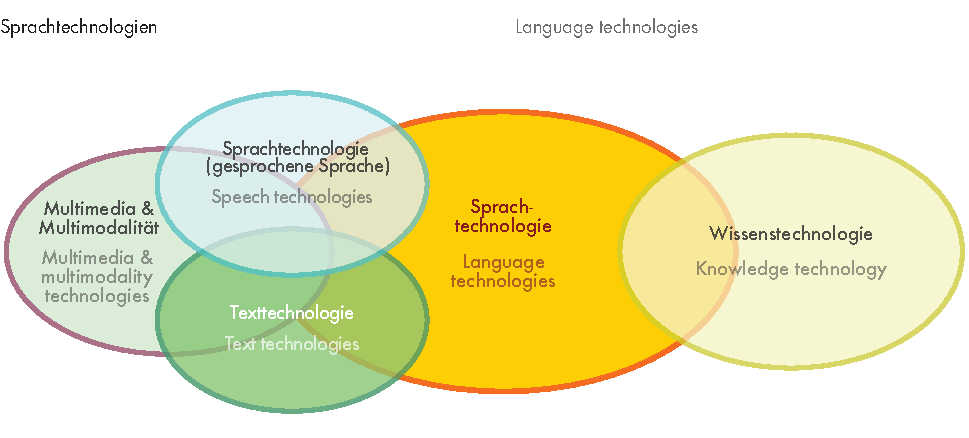
\includegraphics[width=\textwidth]{../_media/language_technologies}
  \caption{Sprachtechnologie im Kontext}
  \label{fig:ltincontext}
  \colorrule{grey3}{\textwidth}{1.5pt}
\end{figure}

Wenn wir kommunizieren, kombinieren wir Sprache mit anderen Kommunikationskanälen und Informationsmedien – Sprechen wird beispielsweise von Gesten und Gesichtsausdrücken begleitet. Text in digitaler Form ist mit Bildern und Tönen verlinkt. Filme können Sprache in gesprochener und geschriebener Form enthalten. Mit anderen Worten, Sprach- und Texttechnologien überlappen und interagieren mit anderen Technologien zur Verarbeitung multimodaler und multimedialer Daten. 

Im Folgenden werden wir uns mit den Hauptanwendungsbereichen der Sprachtechnologie beschäftigen, insbesondere mit Sprachüberprüfung, Websuche, Sprach\-inter\-aktion und maschineller Übersetzung. Dies umfasst Anwendungen und Basistechnologien wie
    \begin{itemize}
      \item Rechtschreibkorrektur
      \item Unterstützung bei der Texterstellung
      \item Computergestützter Spracherwerb
      \item Informationssuche
      \item Informationsextraktion
      \item Textzusammenfassung
      \item Fragenbeantwortungssysteme
      \item Spracherkennung 
      \item Sprachsynthese
    \end{itemize}
Bevor wir die oben genannten Anwendungsbereiche genauer behandeln, werden wir zunächst die Architektur eines typischen sprachtechnologischen Systems beschreiben.


Softwareanwendungen für die Sprachverarbeitung bestehen typischerweise aus mehreren Komponenten, die verschiedene Aspekte der Sprache widerspiegeln. Abbildung \ref{fig:textprocessingarch} zeigt die stark vereinfachte Architektur eines typischen Textverarbeitungssystems. Die ersten drei Module verarbeiten die Struktur und Bedeutung der Texteingabe:
    \begin{enumerate}
      \item Vorverarbeitung: bereinigt die Daten, analysiert oder entfernt Formatierung, ermittelt die Eingabesprache usw.
      \item Grammatikanalyse: findet das Verb, seine Objekte, Modifikatoren, etc. und ermittelt die Satzstruktur.
      \item Semantische Analyse: disambiguiert mehrdeutige Begriffe (d. h. ermittelt die passende Bedeutung von Wörtern in einem bestimmten Kontext); löst Anaphern auf (d. h. welche Pronomen sich auf welche Nomen im Satz beziehen); stellt die Bedeutung des Satzes in maschinenlesbarer Form dar.
    \end{enumerate}
Nach der Analyse des Textes können aufgabenspezifische Module weitere Operationen ausführen, beispielsweise eine automatische Zusammenfassung und oder eine Datenbanksuche. 

\begin{figure}[h!]
  \colorrule{grey3}{\textwidth}{1.5pt}
  \center
  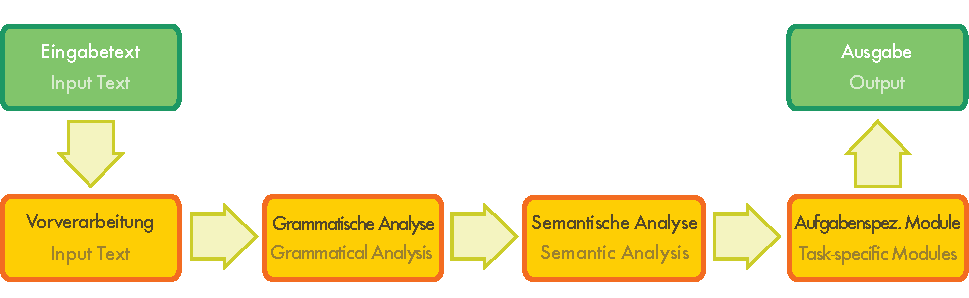
\includegraphics[width=\textwidth]{../_media/text_processing_app_architecture}
  \caption{Eine typische Architektur zur Verarbeitung von Texten}
  \label{fig:textprocessingarch}
  \colorrule{grey3}{\textwidth}{1.5pt}
\end{figure}

Nach einer Einführung der Kernanwendungsbereiche liefern wir einen Überblick über den heutigen Stand der Forschung und Ausbildung im Bereich Sprachtechnologie, sowie über frühere und heutige Forschungsprogramme. Im Anschluss daran präsentieren wir eine Experteneinschätzung zu zentralen Tools und Ressourcen der Sprachtechnologie im Hinblick auf verschiedene Dimensionen wie Verfügbarkeit, Reifegrad und Qualität. Die allgemeine Situation der Sprachtechnologie für die deutsche Sprache wird in einer Tabelle zusammengefasst. Im Text fett gedruckte Anwendungen und Ressourcen sind auch in dieser Tabelle zu finden. Im Anschluss wird das Deutsche im Hinblick auf die sprachtechnologische Unterstützung mit anderen Sprachen verglichen, die Gegenstand der vorliegenden Reihe sind.

  
\subsection{Zentrale Anwendungsbereiche} 

In diesem Abschnitt konzentrieren wir uns auf die wichtigsten sprachtechnologischen Anwendungen und Ressourcen und geben einen Überblick über Aktivitäten im Bereich Sprachtechnologie in Deutschland, Österreich und in der Schweiz. 


\subsubsection{Sprachüberprüfung}

\begin{figure}[h!]
  \colorrule{grey3}{\textwidth}{1.5pt}
  \center
  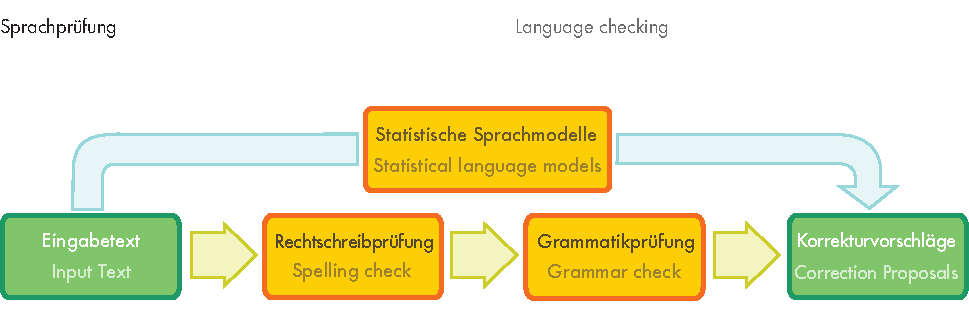
\includegraphics[width=\textwidth]{../_media/language_checking}
  \caption{Sprachüberprüfung (statistisch; regelbasiert)}
  \label{fig:langcheckingaarch}
  \colorrule{grey3}{\textwidth}{1.5pt}
\end{figure}

Jeder, der ein Textverarbeitungsprogramm wie Microsoft Word einsetzt, weiß, dass es eine Rechtschreibprüfung besitzt, die Rechtschreibfehler kenntlich macht und Korrekturen vorschlägt. Die ersten Rechtschreibkorrekturprogramme verglichen eine Liste extrahierter Wörter mit einem Wörterbuch mit richtig geschriebenen Wörtern. Heute sind diese Programme wesentlich ausgefeilter. Mithilfe von sprachabhängigen Algorithmen für die \textbf{Grammatikanalyse} erkennen sie Fehler im Hinblick auf Morphologie (z.\,B., Pluralbildung) sowie syntaxbezogene Fehler, beispielsweise ein fehlendes Verb oder eine fehlende Übereinstimmung zwischen Subjekt und konjugiertem Verb (z.\,B.~\textit{Er *schreiben einen Brief}). Die meisten Rechtschreibprüfungen finden jedoch im folgenden Text keinen Fehler:

Um derartige Fehler zu finden, ist in der Regel eine Analyse des Kontextes notwendig. Beispiel: Ob ein Wort im Deutschen groß oder klein geschrieben werden muss:

\begin{center}
  \begin{tabulary}{150mm}{L} \addlinespace
    \textit{Sie übersetzte den Text ins \textbf{Englische}.}\\ 
    \textit{ {[}She translated the text into English.{]} }\\ 
    \textit{Er las das \textbf{englische} Buch.}\\ 
    \textit{ {[}He read the English book.{]}}\\ 
  \end{tabulary}
\end{center}

Diese Art der Analyse muss entweder auf sprachspezifische \textbf{Grammatiken} zurückgreifen, die von Fachleuten aufwändig in Software kodiert werden, oder auf ein statistisches Sprachmodell. In diesem Fall berechnet ein Modell die Wahrscheinlichkeit eines Wortes an einer bestimmten Position (z.\,B.~zwischen den davor und dahinter stehenden Wörtern). Zum Beispiel ist die Wortfolge \textit{englische Buch} eine wesentlich wahrscheinlichere Wortfolge als \textit{Englisch Buch}. Ein statistisches Sprachmodell kann aus einer großen Menge an (korrekten) Sprachdaten, einem sogenannten \textbf{Textkorpus}, automatisch erstellt werden. Diese Ansätze wurden üblicherweise rund um Daten aus dem Englischen entwickelt. Sie lassen sich nur schwer auf das Deutsche übertragen, weil diese Sprache eine flexible Wortstellung besitzt, Wörter sich beliebig zu Komposita zusammensetzen lassen und es wesentlich mehr Flexion gibt.\\ 
Sprachprüfung ist nicht auf Textverarbeitungssysteme beschränkt. Sie findet auch bei Systemen zur Autorenunterstützung Anwendung, d.\,h. in Softwareumgebungen, in denen nach bestimmten Standards Handbücher und andere Dokumentation für z.\,B.~komplexe IT oder das Gesundheitswesen geschrieben werden. Aus Angst vor Kundenbeschwerden über unsachgemäße Anwendung und Schadensersatzforderungen aufgrund falsch verstandener Anweisungen konzentrieren sich Unternehmen verstärkt auf die Qualität ihrer technischen Dokumentation. Gleichzeitig sprechen sie den internationalen Markt an (mit Übersetzung oder Lokalisierung). Fortschritte in der Verarbeitung natürlicher Sprache haben zur Entwicklung von Software zur Autorenunterstützung geführt. Diese hilft dem Verfasser technischer Dokumentation bei der Verwendung von Wörtern und Satzstrukturen, die den Branchenregeln und terminologischen Beschränkungen der Unternehmen entsprechen.

Einige deutsche Unternehmen und Sprachdienstleister bieten Produkte in diesem Bereich an. Siemens hat mit \textit{Siemens-Dokumentationsdeutsch} eine kontrollierte Sprache für Deutsch zur Verfügung gestellt. IAI, ein deutsches Forschungsinstitut, hat ein Prüfmodul, CLAT, für deutsche Grammatik und Stil entwickelt. Acrolinx, ein deutsches Unternehmen, bietet Software mit einer hochgradig anpassbaren Sprachprüfung sowie einer Terminologiedatenbank an. Die Styleguides von Acrolinx für technische Dokumentation raten vom Gebrauch komplexer zusammengesetzter Substantive wie \textit{Achsmesshebebühne} und metaphorischer Sprache wie \textit{blitzschnell} oder \textit{Faustregel} sowie vom Gebrauch des unpersönlichen Pronomens \textit{man} (z.\,B.~in \textit{Danach stellt man die Maschine aus}) ab. Lange Sätze und Schachtelsätze sollten ebenfalls vermieden werden, weil der Mensch aufgeblähte Sprachkonstrukte nicht so schnell und präzise verarbeiten kann. Auch für maschinelle Übersetzungssysteme wird damit eine gute Übersetzung erschwert.

Neben Rechtschreibprüfungen und Autorenunterstützung spielt die Sprachüberprüfung auch im Bereich des computergestützten Sprachlernens eine Rolle. Außerdem korrigieren Sprachprüfanwendungen automatisch Anfragen bei Suchmaschinen, zum Beispiel bei den Google-Vorschlägen \textit{Meinten Sie…}.


\subsubsection{Websuche}

\begin{figure}[h!]
  \colorrule{grey3}{\textwidth}{1.5pt}
  \center
  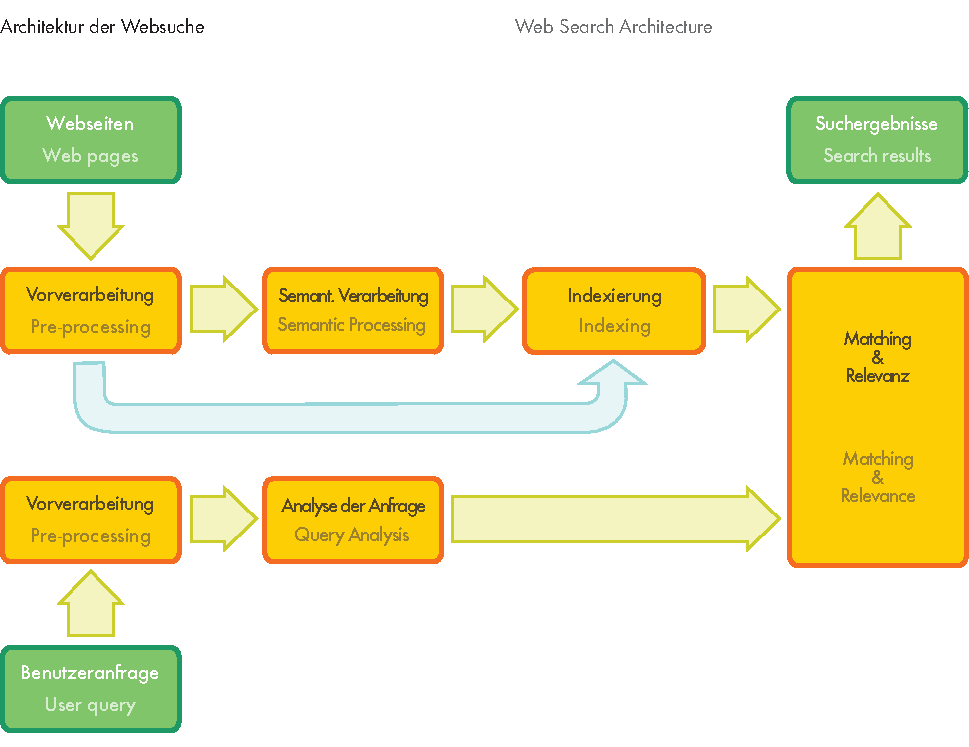
\includegraphics[width=\textwidth]{../_media/web_search_architecture}
  \caption{Websuche}
  \label{fig:websearcharch}
  \colorrule{grey3}{\textwidth}{1.5pt}
\end{figure}

Die Suche im Web, in Intranets oder digitalen Bibliotheken ist wohl die am weitesten verbreitete, doch derzeit noch stark unterentwickelte Sprachtechnologieanwendung. Die 1998 online geschaltete Google-Suchmaschine wickelt heutzutage rund 80\% aller Suchanfragen ab \cite{spi1}. Seit 2004 ist das Verb \textit{googeln} sogar im Duden eingetragen. Die Darstellungsform der Google-Suchoberfläche und der Ergebnisseite hat sich seit der ersten Version nur unwesentlich verändert. In der heutigen Version bietet Google jedoch eine Rechtschreibkorrektur für falsch geschriebene Wörter, sowie semantik-orientierte Suchfunktionen, die die Suchgenauigkeit erhöhen können, indem sie die Bedeutung von Begriffen in ihrem Suchanfragekontext analysieren \cite{pc1}. Die Erfolgsgeschichte von Google zeigt, dass eine große Menge verfügbarer Daten und effiziente Indizierungstechniken mit einem auf Statistik basierenden Ansatz bereits zufriedenstellende Ergebnisse liefern können. 

Für komplexere Informationsanfragen ist es jedoch wichtig, tiefgreifenderes linguistisches Wissen einzubeziehen, um die Anfrage interpretieren zu können. Experimente mit \textbf{lexikalischen Ressourcen} wie maschinenlesbaren Thesauri oder ontologischen Sprachressourcen (z.\,B.~WordNet für Englisch oder GermaNet für Deutsch) haben gezeigt, dass sich das Suchergebnis verbessern lässt, indem die Anfrage um Synonyme oder andere mit dem ursprünglichen Suchbegriff verwandte Begriffe erweitert wird, beispielsweise der Suchbegriff \textit{Atomkraft} um die Begriffe \textit{Kernenergie} und \textit{Nuklearenergie}. 

\boxtext{Die nächste Generation der Suchmaschinen muss noch wesentlich ausgefeiltere Sprachtechnologie enthalten.}Die nächste Generation der Suchmaschinen muss noch wesentlich ausgefeiltere Sprachtechnologie enthalten, insbesondere um mit Suchanfragen zurechtzukommen, die aus einer Frage oder einem vollständigen Satz statt einer Liste von Stichwörtern bestehen. Für die Anfrage \textit{Ich möchte eine Liste aller Unternehmen, die in den vergangenen fünf Jahren von anderen Unternehmen übernommen wurden} ist neben der syntaktischen auch eine \textbf{semantische Analyse} erforderlich. Außerdem muss das System einen Index für den schnellen Abruf einschlägiger Dokumente bereitstellen. Eine zufriedenstellende Antwort erfordert syntaktisches Parsing für die Analyse der grammatikalischen Satzstruktur und um festzustellen, dass der Anwender nach Unternehmen sucht, die übernommen wurden, und nicht nach Unternehmen, die andere Unternehmen übernommen haben. Für den Ausdruck \textit{in den vergangenen fünf Jahren} muss das System -- basierend auf dem aktuellen Jahr -- die entsprechenden Jahre ermitteln. Außerdem muss die Anfrage mit einer riesigen Menge unstrukturierter Daten abgeglichen werden, um die Information zu finden, die der Anwender wünscht. Das Durchsuchen und Einstufen relevanter Dokumente bezeichnet man als Information Retrieval. Um eine Liste der Unternehmen zu generieren, muss das System außerdem eine bestimmte Wortfolge in einem Dokument als Firmenname erkennen.  

Eine noch größere Herausforderung stellt der Abgleich der Anfrage in einer Sprache mit Dokumenten in einer anderen Sprache dar. Das sprachübergreifende Information Retrieval beinhaltet die automatische Übersetzung der Anfrage in alle möglichen Quellsprachen und die anschließende Rückübersetzung der Ergebnisse in die Zielsprache des Benutzers. 

Nachdem heutzutage immer mehr Daten in nicht textueller Form vorliegen, sind Dienste erforderlich, die eine Abfrage multimedialer Informationen durch eine Suche von Bildern, Audiodateien und Videodaten ermöglichen. Bei Audio- und Videodateien muss der Sprachinhalt von einem Spracherkennungsmodul in Text (oder in eine phonetische Darstellung) umgewandelt werden, damit anschließend ein Abgleich mit der Anfrage des Nutzers möglich ist.

In Deutschland haben kleine und mittelgroße Unternehmen wie Neofonie Suchtechnologien entwickelt und bringen diese erfolgreich zur Anwendung. So entstand unter anderem die erste deutsche Websuchmaschine (Fireball), die 1997 online geschaltet wurde und später von Lycos Europe aufgekauft und zu einem Content-Portal weiterentwickelt wurde. Heute bieten nur wenige deutsche Unternehmen wie Neofonie oder die Attensity Group (früher Empolis) eigene Suchmaschinen an. Unternehmen, die an einer Infrastruktur für grundlegende Suchfunktionen interessiert sind, setzen häufig Open-Source-Technologie wie Lucene und Solr ein. Andere Unternehmen setzen auf internationale Suchtechnologien wie FAST (ein norwegisches Unternehmen, das 2008 von Microsoft übernommen wurde) oder Exalead (ein französisches Unternehmen, das 2010 von Dassault Systèmes aufgekauft wurde).

Diese Unternehmen konzentrieren sich auf die Bereitstellung von Add-Ons und erweiterten Suchmaschinen für Special-Interest-Portale. Dabei findet eine themen-spezifische Semantik Anwendung. Aufgrund der hohen Anforderungen an Rechenleistung sind solche Suchmaschinen nur kosteneffektiv, wenn damit verhältnismäßig kleine Textmengen verarbeitet werden. Die Verarbeitung dauert zigtausend mal so lange wie bei einer üblichen statistischen Suchmaschine wie Google. Für die themenspezifische Domänenmodellierung sind diese Suchmaschinen zwar sehr gefragt, im Web mit seinen Milliarden und Abermilliarden von Dokumenten lassen sie sich jedoch nicht einsetzen.

MetaGer ist eine Metasuchmaschine, die von der Universität Hannover betrieben wird. Intrafind, ein in München ansässiges Unternehmen, und andere Unternehmen haben sich auf Intranet-Suchanwendungen und Suchanwendungen für Produkte wie SAP spezialisiert, bei denen eine Anpassung an bestimmte Kundendaten erforderlich ist. In der Schweiz liefert Eurospider eine Informationssuche für Internet-Portale. In Österreich gibt es Websuchmaschinen speziell für österreichische Websites wie AT:SEARCH, AUSTRIA-SEEK oder AUSTROLINKS, ihre Abdeckung und Reichweite sind jedoch begrenzt. Neben diesen Suchmaschinen haben österreichische Unternehmen Suchmaschinen für besondere Zwecke entwickelt, beispielsweise 123people, eine Anwendung zur Personensuche in Echtzeit, die die regionale und internationale Suche z.\,B.~für Österreich, Deutschland, Kanada, die USA und GB unterstützt, oder Tripwolf, eine Onlinereiseplattform.
  

\subsubsection{Sprachliche Interaktion}

Sprachliche Interaktion ist eine der vielen Anwendungsbereiche, die auf Technologien zur Verarbeitung gesprochener Sprache zurück greift. Der Technologiebereich sprachliche Interaktion dient zur Schaffung von Schnittstellen, über die Nutzer in gesprochener Sprache interagieren können, statt über eine grafische Anzeige, Tastatur und Maus. Heute finden diese sprachbasierten Benutzerschnittstellen (engl. Voice User Interfaces, VUI) bei teil- oder vollautomatischen Telefondiensten Anwendung, die Unternehmen ihren Kunden, Mitarbeitern oder Partnern anbieten. Geschäftsdomänen, die VUIs verstärkt einsetzen, sind beispielsweise Banken, Lieferketten, das öffentliche Transportwesen und Telekommunikationsunternehmen. Weitere Anwendungen für die Verarbeitung gesprochener Sprache sind Schnittstellen zu Kfz-Navigationssystemen sowie der Einsatz gesprochener Sprache als Alternative zu grafischen Oberflächen oder Touchscreens in Smartphones.

\begin{figure}[h!]
  \colorrule{grey3}{\textwidth}{1.5pt}
  \center 
  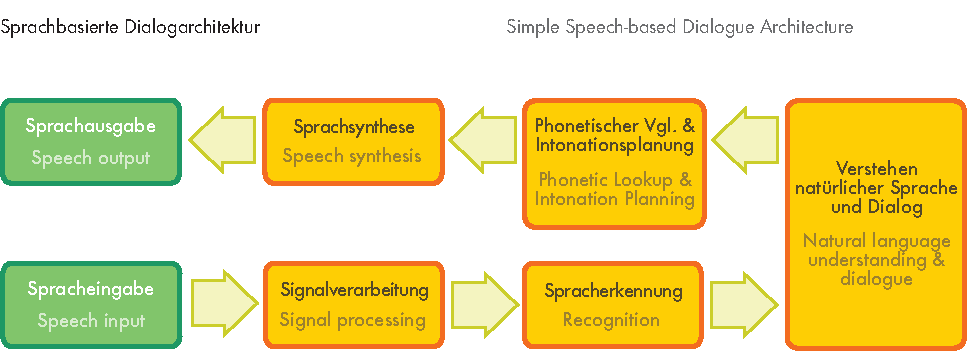
\includegraphics[width=\textwidth]{../_media/simple_speech-based_dialogue_architecture}
  \caption{Sprachdialogsystem}
  \label{fig:dialoguearch}
  \colorrule{grey3}{\textwidth}{1.5pt}
\end{figure}

Technologien zur Verarbeitung gesprochener Sprache setzen sich aus vier Bereichen zusammen:

\begin{enumerate}
  \item Automatische \textbf{Spracherkennung} (ASR) bestimmt, welche Wörter in einer vom Benutzer geäußerten Lautabfolge tatsächlich gesprochen werden.
  \item Sprachverarbeitung analysiert die syntaktische Struktur der Äußerung des Benutzers und interpretiert sie dem jeweiligen System entsprechend.
  \item Dialogverwaltung bestimmt, basierend auf der Benutzereingabe, welche Systemfunktionalität aufgerufen werden muss.    
  \item \textbf{Sprachsynthese} (Text-to-Speech oder TTS) wandelt die Antwort des Systems in gesprochene Sprache um.
\end{enumerate}

Eine der größten Herausforderungen von ASR-Syste\-men besteht in der genauen Erkennung der Wortabfolge, die ein Nutzer ausspricht. Hierfür muss entweder der Bereich der möglichen, vom Nutzer ausgesprochenen Wörter auf eine begrenzte Zahl von Stichwörtern beschränkt werden oder es müssen manuelle  Sprachmodelle erstellt werden, die eine Vielzahl von Äußerungen abdecken. Mithilfe von Techniken des maschinellen Lernens können Sprachmodelle auch automatisch aus großen Ansammlungen von Sprachaudiodateien und Texttranskriptionen, sogenannten \textbf{Sprachkorpora}, erzeugt werden. Eine Einschränkung der möglichen Äußerungen schränkt den Nutzer der sprachlichen Benutzerschnittstelle stark ein, was sich nachteilig auf die Akzeptanz auswirken kann. Die Schaffung und Verwaltung vielfältiger Sprachmodelle ist jedoch mit beträchtlichen Kosten verbunden. VUIs, die Sprachmodelle einsetzen und es dem Nutzer anfangs gestatten, sein Anliegen etwas flexibler auszudrücken -- über die Begrüßungsfloskel \textit{Wie kann ich Ihnen helfen?} --, sind häufig automatisiert und werden von den Nutzern eher angenommen. 

Unternehmen verwenden oftmals Aufzeichnungen von professionellen Sprechern für die Ausgabe von sprachlichen Benutzerschnittstellen. Für statische Äußerungen, bei denen der Wortlaut nicht von einem bestimmten Kontext oder persönlichen Nutzerdaten abhängt, kann dies eine sehr gutes Nutzerempfinden mit sich bringen. Aber dynamischerer Inhalt in einer Äußerung kann unter Umständen durch eine unnatürliche Intonation beeinträchtigt werden, da einzelne Audiodateien einfach zusammengefügt wurden. TTS-Systeme werden jedoch zunehmend besser darin, natürlich klingende dynamische Äußerungen zu produzieren, wobei noch immer Verbesserungsbedarf besteht. 

Die auf dem Markt erhältlichen Schnittstellen zur Verarbeitung gesprochener Sprache wurden in den letzten zehn Jahren im Hinblick auf ihre verschiedenen Technologiekomponenten beträchtlich standardisiert. Auch hat in der Spracherkennung und Sprachsynthese eine starke Marktkonsolidierung stattgefunden. Die Binnenmärkte in den G20-Ländern (wirtschaftlich starke Länder mit hohen Bevölkerungszahlen) werden von gerade einmal fünf globalen Playern dominiert, von denen Nuance (USA) und Loquendo (Italien) in Europa die Vormachtstellung haben. 2011 gab Nuance die Übernahme von Loquendo bekannt, was einen weiteren Schritt zur Marktkonsolidierung darstellt.

Auf dem deutschsprachigen TTS-Markt gibt es kleinere Unternehmen wie voiceINTERconnect und Ivona. Die Schweizer Firma SVOX wurde 2011 von Nuance übernommen. Eine Österreichisch-Deutsche TTS-Sprache wurde 2010 von CereProc, einem britischen Unternehmen, kommerzialisiert. Viele Jahre lang unterhielt Philips Speech Recognition Systems eine starke ASR-Forschungs- und Entwicklungseinheit in Österreich, die 2008 von Nuance übernommen wurde. Heute ist Simon Listens eine gemeinnützige österreichische Organisation, die Open-Source-ASR-Software entwickelt und sich dabei auf Anwendungen für Benutzergruppen mit besonderen Anforderungen konzentriert, wie Körperbehinderte und ältere Menschen.

Im Hinblick auf Technologie und Knowhow im Bereich Dialogverwaltung wird der Markt von nationalen KMU-Playern dominiert. In Deutschland gehören dazu Crealog, Excelsis und SemanticEdge. Statt auf ein Geschäft mit Produkten auf Basis von Softwarelizenzen zu setzen, sind diese Unternehmen überwiegend Vollserviceanbieter, die sprachliche Benutzerschnittstellen als Teil ihres Systemintegrationsdienstes entwickeln. Im Bereich der Sprachein- und Ausgabe gibt es bisher noch keinen echten Markt für Kerntechnologien, die auf syntaktischer und semantischer Analyse basieren.

In den vergangenen fünf Jahren ist die Nachfrage nach sprachlichen Benutzerschnittstellen in Deutschland rasant gestiegen, vor allem aufgrund der zunehmenden Nachfrage nach Kunden-Self-Service, Kostenoptimierung für automatische Telefondienste und die wachsende Akzeptanz gesprochener Sprache als Medium für die Interaktion zwischen Mensch und Maschine. All dies wurde durch die Schaffung des Netzwerks www.voice-community.de katalysiert, das Akteure aus der Industrie, Forschungsinstitute und Unternehmenskunden zusammenbrachte. Neben weiteren Errungenschaften brachte es einen gemeinsamen Plan für VUI-Qualität an den Start und organisierte die jährlich abgehaltene Veranstaltung VOICE Days mit einem Wettbewerb, bei dem in verschiedenen Kategorien VOICE-Awards vergeben wurden. Als akademische Partner spielten das DFKI und das Fraunhofer IAO-Institut eine wichtige Rolle bei der Verbreitung von Wissen über die Vorteile der Sprachtechnologie in deutsche Unternehmen.

Künftig wird sich aufgrund der Verbreitung von Smartphones als neue Plattform zur Verwaltung von Kundenbeziehungen neben Festnetztelefonen, dem Internet und E-Mail sehr viel ändern. Dies wird sich auch auf den Einsatz der Technologien für gesprochene Sprache auswirken. Langfristig gesehen wird es mehr telefonbasierte VUI geben und gesprochene Sprache wird als benutzerfreundliche Eingabemöglichkeit bei Smartphones eine wesentlich zentralere Rolle spielen. Ausschlaggebend werden dafür vor allem schrittweise Verbesserungen in der Genauigkeit der sprecherunabhängigen Spracherkennung über Diktierdienste sein, die Smartphone-Nutzern bereits heute als zentrale Dienste angeboten werden.


\subsubsection{Maschinelle Übersetzung}

\begin{figure}[h!]
  \colorrule{grey3}{\textwidth}{1.5pt}
  \center
  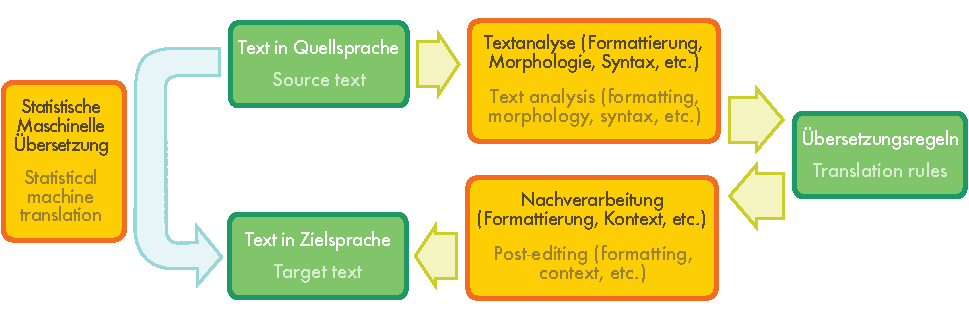
\includegraphics[width=\textwidth]{../_media/machine_translation}
  \caption{Maschinelle Übersetzung (statistisch; regelbasiert)}
  \label{fig:mtarch}
  \colorrule{grey3}{\textwidth}{1.5pt}
\end{figure}

Die Idee, digitale Computer für die Übersetzung natürlicher Sprachen einzusetzen, geht auf das Jahr 1946 zurück. In den 1950er-Jahren und dann wieder in den 1980er-Jahren wurden größere Summen in die entsprechende Forschung investiert. Doch die \textbf{maschinelle Übersetzung} („machine translation“ MT) kann bisher das anfängliche Versprechen einer allgemein verwendbaren automatischen Übersetzung noch nicht halten.\\
Der naheliegendste Ansatz bei der Maschinellen Übersetzung besteht darin, die Wörter eines Textes in der einen Sprache automatisch durch die entsprechenden Wörter in einer anderen Sprache zu ersetzen. In Themengebieten mit sehr beschränkter, formelhafter Sprache, beispielsweise bei Wetterberichten, kann dies zum gewünschten Ergebnis führen. Für eine gute Übersetzung weniger standardisierter Texte müssen jedoch größere Texteinheiten (Phrasen, Sätze oder sogar ganze Abschnitte) den jeweiligen Entsprechungen in der Zielsprache zugeordnet werden. Die größte Schwierigkeit besteht darin, dass die menschliche Sprache vieldeutig ist. Vieldeutigkeit stellt auf mehreren Ebenen eine Herausforderung dar: Auf lexikalischer Ebene muss einem Begriff die passende Bedeutung zugeordnet werden (ist \textit{Jaguar} eine Automarke oder ein Tier?), auf syntaktischer Ebene kann die Fallzuweisung eine Schwierigkeit darstellen, beispielsweise in:

\begin{center}
  \begin{tabulary}{150mm}{L} \addlinespace
  \textit{Die Frau sah das Auto und \textbf{ihr} Mann auch.}\\ 
  \textit{Die Frau sah das Auto und \textbf{ihren} Mann auch. }\\ 
  \textit{[The woman saw the car and her husband, too.]}\\ 
  \end{tabulary}
\end{center}

Ein MT-System lässt sich zum einen mithilfe linguistischer Regeln aufbauen. Für Übersetzungen zwischen nahe verwandten Sprachen kann eine wörtliche Übersetzung wie in dem o.g. Beispiel praktikabel sein. Regelbasierte, durch linguistisches Wissen gesteuerte Systeme analysieren jedoch oft den eingegebenen Text und erstellen eine symbolische Zwischendarstellung, aus welcher der Text in die Zielsprache übertragen werden kann. Der Erfolg dieser Methoden hängt weitgehend von der Verfügbarkeit umfassender Lexika mit morphologischen, syntaktischen und semantischen Informationen sowie umfangreichen Grammatikregelsätzen ab, die von qualifizierten Linguistiken mit großer Sorgfalt entworfen werden. Das ist ein sehr langer und damit kostspieliger Prozess.

In den späten 1980er-Jahren, als die Computerrechenleistung zunahm und billiger wurde, wuchs das Interesse an statistischen Modellen für die maschinelle Übersetzung. Statistische Modelle werden aus der Analyse mehrsprachiger Textdaten, sogenannter \textbf{paralleler Korpora}, abgeleitet, z.\,B.~dem Parallelkorpus Europarl, der die Verfahren des Europäischen Parlaments in 11 europäischen Sprachen umfasst. Wenn ausreichend Daten zur Verfügung stehen, funktioniert statistische MT gut genug, um eine ungefähre Bedeutung eines Textes in einer Fremdsprache durch die Verarbeitung paralleler Versionen und Ermittlung plausibler Wortmuster abzuleiten. Aber im Gegensatz zu wissensgestützten Systemen produziert die statistische (oder datengetriebene) MT häufig grammatikalisch fehlerhafte Ergebnisse. Ein Vorteil der datengetriebenen MT ist, dass weniger Aufwand durch den Menschen erforderlich ist. Sie kann außerdem spezielle sprachliche Besonderheiten abdecken (z.\,B.~idiomatische Ausdrücke), die bei wissensgesteuerten Systemen oft außer Acht gelassen werden. 

Die Stärken und Schwächen der wissensgesteuerten und datengetriebenen Systeme zur maschinellen Übersetzung ergänzen sich häufig, sodass sich die Forschung heutzutage auf hybride Ansätze konzentriert, die beide Methoden kombinieren (vergleiche den Abschnitt zu „Spracherwerb bei Menschen und Maschinen“ für weitere Informationen zum Thema). Eine Möglichkeit besteht darin, wissens- und datengesteuerte Systeme mit einem Auswahlmodul zu verbinden, das bei jedem Satz das beste Ergebnis bestimmt. Die Ergebnisse sind jedoch bei längeren Sätzen (mit mehr als ca. 12 Wörtern) oftmals weit davon entfernt, perfekt zu sein. Eine bessere Lösung ist die Kombination der besten Teile jeden Satzes aus mehreren Ergebnissen. Das kann eine ziemlich komplexe Aufgabe werden, da die entsprechenden Teile mehrerer Alternativen nicht immer offensichtlich sind und aufeinander abgestimmt werden müssen. 

Maschinelle Übersetzung stellt besonders bei der deutschen Sprache eine große Herausforderung dar.

\boxtext{Maschinelle Übersetzung stellt besonders bei der deutschen Sprache eine große Herausforderung dar.} Die Möglichkeit der beliebigen Wortneuschöpfung durch das Verbinden von Wörtern erschwert die Wortanalyse und die Erstellung von Wörterbüchern. Eine frei wählbare Wortstellung und getrennte Verbkonstruktionen können bei der Satzanalyse zu Problemen führen. Die umfangreiche Flexion stellt eine Herausforderung dar, wenn Wörter mit richtigem Geschlecht und im richtigen Fall gebildet werden müssen. 

Einige der wichtigsten bestehenden MT-Systeme wurden in Deutschland entwickelt und hier zur Marktreife gebracht. Hierzu zählen LOGOS, METAL (Siemens) und LMT (IBM Heidelberg). Als diese Unternehmen ihr anfängliches Engagement für die Entwicklung dieser Technologie einstellten, wurde die Entwicklung auf Geschäftsausgliederungen übertragen. LOGOS wurde als Open-Source System zur Verfügung gestellt. METAL wurde von GMS und später von Lucy Software übernommen und auf dem Einzelhandelsmarkt auch als Langenscheidt T1 angeboten. Das IBM-System bildet die Grundlage für Produktangebote von Linguatec (Personal Translator) und Lingenio (translate). CLS Communication bietet MT in der Schweiz an. Alle diese Systeme arbeiten regelbasiert. Obwohl viel Forschungsarbeit auf nationaler und internationaler Ebene im Bereich dieser Technologie geleistet wird, sind hybride Systeme bisher bei professionellen Anwendungen wesentlich weniger erfolgreich als im Forschungslabor. 

Der Einsatz maschineller Übersetzung kann die Produktivität erheblich steigern, sofern das System in intelligenter Weise an die benutzerspezifische Terminologie angepasst und in die Arbeitsabläufe integriert wird. Spezielle Systeme für interaktive Übersetzungsunterstützung wurden beispielsweise von Siemens entwickelt. Sprachportale wie die Website von Volkswagen bieten Zugriff auf Wörterbücher, firmenspezifische Terminologie, gespeicherte Übersetzungen und Unterstützung durch MT. 

Bezüglich der Qualität von MT-Systemen besteht noch riesiges Verbesserungspotenzial. Zu den Herausforderungen gehören die Anpassung von Sprachressourcen an ein bestimmtes Themengebiet oder einen Anwendungsbereich sowie die Integration der Technologie in Arbeitsabläufe, bei denen bereits mit Terminologiedatenbanken und Übersetzungsspeichern gearbeitet wird. Ein weiteres Problem liegt darin, dass die meisten der aktuellen Systeme auf dem Englischen basieren und nur für wenige Sprachen eine Übersetzung aus dem Deutschen und in das Deutsche unterstützen. Dies führt zu Reibung bei den Übersetzungsarbeitsabläufen und zwingt Anwender der MT, verschiedene Lexikonkodierungstools für verschiedene Systeme zu erlernen.

Anhand von Evaluationskampagnen lassen sich die Qualität von MT-Systemen, die verschiedenen Ansätze und der Status der Systeme für verschiedene Sprachenpaare vergleichen. Tabelle X, die im Rahmen des EU-Projekts Euromatrix+ erstellt wurde, zeigt die Ergebnisse für die Sprachpaare von 22 der 23 Amtssprachen der EU (Irisch wurde nicht in den Vergleich aufgenommen). Die Ergebnisse baieren auf BLEU-Punktewerten \cite{bleu1}. BLEU ist eine automatisierte Evaluationsmethode, die grobe Hinweise auf die Qualität der Übersetzung liefert; bessere Übersetzungen erhalten mehr Punkte. Ein menschlicher Übersetzer würde etwa 80 Punkte erzielen.

Die besten Ergebnisse (in grün und blau) wurden von Sprachen erreicht, bei denen beträchtliche Forschungsarbeit in koordinierte Programme gesteckt wurde und die über viele Parallelkorpora verfügen (z.\,B.~Englisch, Französisch, Niederländisch, Spanisch und Deutsch). Die Sprachen mit schlechteren Ergebnissen sind rot dargestellt. Bei diesen Sprachen mangelt es entweder an entsprechender Entwicklungsarbeit, oder sie unterscheiden sich strukturell erheblich von anderen Sprachen (z.\,B.~Ungarisch, Maltesisch und Finnisch).

\begin{sidewaysfigure}
  \centering
  \setlength{\tabcolsep}{0.4em}
  \begin{tabular}{>{\columncolor{orange1}}cccccccccccccccccccccccc}
      \small
    & \multicolumn{22}{>{\columncolor{orange1}}c}{Zielsprache -- Target Language}\\\addlinespace[{-.009cm}]
    \rowcolor{orange1}  & EN & BG & DE & CS & DA & EL & ES & ET & FI & FR & HU & IT & LT & LV & MT & NL & PL & PT & RO & SK & SL & SV\\
    EN & -- & \textcolor{blue}{40.5} & \textcolor{blue}{46.8} & \textcolor{green2}{52.6} & \textcolor{green2}{50.0} & \textcolor{blue}{41.0} & \textcolor{green2}{55.2} & \textcolor{purple}{34.8} & \textcolor{purple}{38.6} & \textcolor{green2}{50.1} & \textcolor{purple}{37.2} & \textcolor{green2}{50.4} & \textcolor{purple}{39.6} & \textcolor{blue}{43.4} & \textcolor{purple}{39.8} & \textcolor{green2}{52.3} & \textcolor{blue}{49.2} & \textcolor{green2}{55.0} & \textcolor{blue}{49.0} & \textcolor{blue}{44.7} & \textcolor{green2}{50.7} & \textcolor{green2}{52.0}\\
    BG & \textcolor{green}{61.3} & -- & \textcolor{purple}{38.7} & \textcolor{purple}{39.4} & \textcolor{purple}{39.6} & \textcolor{purple}{34.5} & \textcolor{blue}{46.9} & \textcolor{red3}{25.5} & \textcolor{red3}{26.7} & \textcolor{blue}{42.4} & \textcolor{red3}{22.0} & \textcolor{blue}{43.5} & \textcolor{red3}{29.3} & \textcolor{red3}{29.1} & \textcolor{red3}{25.9} & \textcolor{blue}{44.9} & \textcolor{purple}{35.1} & \textcolor{blue}{45.9} & \textcolor{purple}{36.8} & \textcolor{purple}{34.1} & \textcolor{purple}{34.1} & \textcolor{purple}{39.9}\\
    DE & \textcolor{green2}{53.6} & \textcolor{red3}{26.3} & -- & \textcolor{purple}{35.4} & \textcolor{blue}{43.1} & \textcolor{purple}{32.8} & \textcolor{blue}{47.1} & \textcolor{red3}{26.7} & \textcolor{red3}{29.5} & \textcolor{purple}{39.4} & \textcolor{red3}{27.6} & \textcolor{blue}{42.7} & \textcolor{red3}{27.6} & \textcolor{purple}{30.3} & \textcolor{red2}{19.8} & \textcolor{green2}{50.2} & \textcolor{purple}{30.2} & \textcolor{blue}{44.1} & \textcolor{purple}{30.7} & \textcolor{red3}{29.4} & \textcolor{purple}{31.4} & \textcolor{blue}{41.2}\\
    CS & \textcolor{green2}{58.4} & \textcolor{purple}{32.0} & \textcolor{blue}{42.6} & -- & \textcolor{blue}{43.6} & \textcolor{purple}{34.6} & \textcolor{blue}{48.9} & \textcolor{purple}{30.7} & \textcolor{purple}{30.5} & \textcolor{blue}{41.6} & \textcolor{red3}{27.4} & \textcolor{blue}{44.3} & \textcolor{purple}{34.5} & \textcolor{purple}{35.8} & \textcolor{red3}{26.3} & \textcolor{blue}{46.5} & \textcolor{purple}{39.2} & \textcolor{blue}{45.7} & \textcolor{purple}{36.5} & \textcolor{blue}{43.6} & \textcolor{blue}{41.3} & \textcolor{blue}{42.9}\\
    DA & \textcolor{green2}{57.6} & \textcolor{red3}{28.7} & \textcolor{blue}{44.1} & \textcolor{purple}{35.7} & -- & \textcolor{purple}{34.3} & \textcolor{blue}{47.5} & \textcolor{red3}{27.8} & \textcolor{purple}{31.6} & \textcolor{blue}{41.3} & \textcolor{red3}{24.2} & \textcolor{blue}{43.8} & \textcolor{red3}{29.7} & \textcolor{purple}{32.9} & \textcolor{red3}{21.1} & \textcolor{blue}{48.5} & \textcolor{purple}{34.3} & \textcolor{blue}{45.4} & \textcolor{purple}{33.9} & \textcolor{purple}{33.0} & \textcolor{purple}{36.2} & \textcolor{blue}{47.2}\\
    EL & \textcolor{green2}{59.5} & \textcolor{purple}{32.4} & \textcolor{blue}{43.1} & \textcolor{purple}{37.7} & \textcolor{blue}{44.5} & -- & \textcolor{green2}{54.0} & \textcolor{red3}{26.5} & \textcolor{red3}{29.0} & \textcolor{blue}{48.3} & \textcolor{red3}{23.7} & \textcolor{blue}{49.6} & \textcolor{red3}{29.0} & \textcolor{purple}{32.6} & \textcolor{red3}{23.8} & \textcolor{blue}{48.9} & \textcolor{purple}{34.2} & \textcolor{green2}{52.5} & \textcolor{purple}{37.2} & \textcolor{purple}{33.1} & \textcolor{purple}{36.3} & \textcolor{blue}{43.3}\\
    ES & \textcolor{green}{60.0} & \textcolor{purple}{31.1} & \textcolor{blue}{42.7} & \textcolor{purple}{37.5} & \textcolor{blue}{44.4} & \textcolor{purple}{39.4} & -- & \textcolor{red3}{25.4} & \textcolor{red3}{28.5} & \textcolor{green2}{51.3} & \textcolor{red3}{24.0} & \textcolor{green2}{51.7} & \textcolor{red3}{26.8} & \textcolor{purple}{30.5} & \textcolor{red3}{24.6} & \textcolor{blue}{48.8} & \textcolor{purple}{33.9} & \textcolor{green2}{57.3} & \textcolor{purple}{38.1} & \textcolor{purple}{31.7} & \textcolor{purple}{33.9} & \textcolor{blue}{43.7}\\
    ET & \textcolor{green2}{52.0} & \textcolor{red3}{24.6} & \textcolor{purple}{37.3} & \textcolor{purple}{35.2} & \textcolor{purple}{37.8} & \textcolor{red3}{28.2} & \textcolor{blue}{40.4} & -- & \textcolor{purple}{37.7} & \textcolor{purple}{33.4} & \textcolor{purple}{30.9} & \textcolor{purple}{37.0} & \textcolor{purple}{35.0} & \textcolor{purple}{36.9} & \textcolor{red3}{20.5} & \textcolor{blue}{41.3} & \textcolor{purple}{32.0} & \textcolor{purple}{37.8} & \textcolor{red3}{28.0} & \textcolor{purple}{30.6} & \textcolor{purple}{32.9} & \textcolor{purple}{37.3}\\
    FI & \textcolor{blue}{49.3} & \textcolor{red3}{23.2} & \textcolor{purple}{36.0} & \textcolor{purple}{32.0} & \textcolor{purple}{37.9} & \textcolor{red3}{27.2} & \textcolor{purple}{39.7} & \textcolor{purple}{34.9} & -- & \textcolor{red3}{29.5} & \textcolor{red3}{27.2} & \textcolor{purple}{36.6} & \textcolor{purple}{30.5} & \textcolor{purple}{32.5} & \textcolor{red2}{19.4} & \textcolor{blue}{40.6} & \textcolor{red3}{28.8} & \textcolor{purple}{37.5} & \textcolor{red3}{26.5} & \textcolor{red3}{27.3} & \textcolor{red3}{28.2} & \textcolor{purple}{37.6}\\
    FR & \textcolor{green}{64.0} & \textcolor{purple}{34.5} & \textcolor{blue}{45.1} & \textcolor{purple}{39.5} & \textcolor{blue}{47.4} & \textcolor{blue}{42.8} & \textcolor{green}{60.9} & \textcolor{red3}{26.7} & \textcolor{purple}{30.0} & -- & \textcolor{red3}{25.5} & \textcolor{green2}{56.1} & \textcolor{red3}{28.3} & \textcolor{purple}{31.9} & \textcolor{red3}{25.3} & \textcolor{green2}{51.6} & \textcolor{purple}{35.7} & \textcolor{green}{61.0} & \textcolor{blue}{43.8} & \textcolor{purple}{33.1} & \textcolor{purple}{35.6} & \textcolor{blue}{45.8}\\
    HU & \textcolor{blue}{48.0} & \textcolor{red3}{24.7} & \textcolor{purple}{34.3} & \textcolor{purple}{30.0} & \textcolor{purple}{33.0} & \textcolor{red3}{25.5} & \textcolor{purple}{34.1} & \textcolor{red3}{29.6} & \textcolor{red3}{29.4} & \textcolor{purple}{30.7} & -- & \textcolor{purple}{33.5} & \textcolor{red3}{29.6} & \textcolor{purple}{31.9} & \textcolor{red2}{18.1} & \textcolor{purple}{36.1} & \textcolor{red3}{29.8} & \textcolor{purple}{34.2} & \textcolor{red3}{25.7} & \textcolor{red3}{25.6} & \textcolor{red3}{28.2} & \textcolor{purple}{30.5}\\
    IT & \textcolor{green}{61.0} & \textcolor{purple}{32.1} & \textcolor{blue}{44.3} & \textcolor{purple}{38.9} & \textcolor{blue}{45.8} & \textcolor{blue}{40.6} & \textcolor{red3}{26.9} & \textcolor{red3}{25.0} & \textcolor{red3}{29.7} & \textcolor{green2}{52.7} & \textcolor{red3}{24.2} & -- & \textcolor{red3}{29.4} & \textcolor{purple}{32.6} & \textcolor{red3}{24.6} & \textcolor{green2}{50.5} & \textcolor{purple}{35.2} & \textcolor{green2}{56.5} & \textcolor{purple}{39.3} & \textcolor{purple}{32.5} & \textcolor{purple}{34.7} & \textcolor{blue}{44.3}\\
    LT & \textcolor{green2}{51.8} & \textcolor{red3}{27.6} & \textcolor{purple}{33.9} & \textcolor{purple}{37.0} & \textcolor{purple}{36.8} & \textcolor{red3}{26.5} & \textcolor{red3}{21.1} & \textcolor{purple}{34.2} & \textcolor{purple}{32.0} & \textcolor{purple}{34.4} & \textcolor{red3}{28.5} & \textcolor{purple}{36.8} & -- & \textcolor{blue}{40.1} & \textcolor{red3}{22.2} & \textcolor{purple}{38.1} & \textcolor{purple}{31.6} & \textcolor{purple}{31.6} & \textcolor{red3}{29.3} & \textcolor{purple}{31.8} & \textcolor{purple}{35.3} & \textcolor{purple}{35.3}\\
    LV & \textcolor{green2}{54.0} & \textcolor{red3}{29.1} & \textcolor{purple}{35.0} & \textcolor{purple}{37.8} & \textcolor{purple}{38.5} & \textcolor{red3}{29.7} & \textcolor{red2}{8.0} & \textcolor{purple}{34.2} & \textcolor{purple}{32.4} & \textcolor{purple}{35.6} & \textcolor{red3}{29.3} & \textcolor{purple}{38.9} & \textcolor{purple}{38.4} & -- & \textcolor{red3}{23.3} & \textcolor{blue}{41.5} & \textcolor{purple}{34.4} & \textcolor{purple}{39.6} & \textcolor{purple}{31.0} & \textcolor{purple}{33.3} & \textcolor{purple}{37.1} & \textcolor{purple}{38.0}\\
    MT & \textcolor{green}{72.1} & \textcolor{purple}{32.2} & \textcolor{purple}{37.2} & \textcolor{purple}{37.9} & \textcolor{purple}{38.9} & \textcolor{purple}{33.7} & \textcolor{blue}{48.7} & \textcolor{red3}{26.9} & \textcolor{red3}{25.8} & \textcolor{blue}{42.4} & \textcolor{red3}{22.4} & \textcolor{blue}{43.7} & \textcolor{purple}{30.2} & \textcolor{purple}{33.2} & -- & \textcolor{blue}{44.0} & \textcolor{purple}{37.1} & \textcolor{blue}{45.9} & \textcolor{purple}{38.9} & \textcolor{purple}{35.8} & \textcolor{blue}{40.0} & \textcolor{blue}{41.6}\\
    NL & \textcolor{green2}{56.9} & \textcolor{red3}{29.3} & \textcolor{blue}{46.9} & \textcolor{purple}{37.0} & \textcolor{blue}{45.4} & \textcolor{purple}{35.3} & \textcolor{blue}{49.7} & \textcolor{red3}{27.5} & \textcolor{red3}{29.8} & \textcolor{blue}{43.4} & \textcolor{red3}{25.3} & \textcolor{blue}{44.5} & \textcolor{red3}{28.6} & \textcolor{purple}{31.7} & \textcolor{red3}{22.0} & -- & \textcolor{purple}{32.0} & \textcolor{blue}{47.7} & \textcolor{purple}{33.0} & \textcolor{purple}{30.1} & \textcolor{purple}{34.6} & \textcolor{blue}{43.6}\\
    PL & \textcolor{green}{60.8} & \textcolor{purple}{31.5} & \textcolor{blue}{40.2} & \textcolor{blue}{44.2} & \textcolor{blue}{42.1} & \textcolor{purple}{34.2} & \textcolor{blue}{46.2} & \textcolor{red3}{29.2} & \textcolor{red3}{29.0} & \textcolor{blue}{40.0} & \textcolor{red3}{24.5} & \textcolor{blue}{43.2} & \textcolor{purple}{33.2} & \textcolor{purple}{35.6} & \textcolor{red3}{27.9} & \textcolor{blue}{44.8} & -- & \textcolor{blue}{44.1} & \textcolor{purple}{38.2} & \textcolor{purple}{38.2} & \textcolor{purple}{39.8} & \textcolor{blue}{42.1}\\
    PT & \textcolor{green}{60.7} & \textcolor{purple}{31.4} & \textcolor{blue}{42.9} & \textcolor{purple}{38.4} & \textcolor{blue}{42.8} & \textcolor{blue}{40.2} & \textcolor{green}{60.7} & \textcolor{red3}{26.4} & \textcolor{red3}{29.2} & \textcolor{green2}{53.2} & \textcolor{red3}{23.8} & \textcolor{green2}{52.8} & \textcolor{red3}{28.0} & \textcolor{purple}{31.5} & \textcolor{red3}{24.8} & \textcolor{blue}{49.3} & \textcolor{purple}{34.5} & -- & \textcolor{purple}{39.4} & \textcolor{purple}{32.1} & \textcolor{purple}{34.4} & \textcolor{blue}{43.9}\\
    RO & \textcolor{green}{60.8} & \textcolor{purple}{33.1} & \textcolor{purple}{38.5} & \textcolor{purple}{37.8} & \textcolor{blue}{40.3} & \textcolor{purple}{35.6} & \textcolor{green2}{50.4} & \textcolor{red3}{24.6} & \textcolor{red3}{26.2} & \textcolor{blue}{46.5} & \textcolor{red3}{25.0} & \textcolor{blue}{44.8} & \textcolor{red3}{28.4} & \textcolor{red3}{29.9} & \textcolor{red3}{28.7} & \textcolor{blue}{43.0} & \textcolor{purple}{35.8} & \textcolor{blue}{48.5} & -- & \textcolor{purple}{31.5} & \textcolor{purple}{35.1} & \textcolor{purple}{39.4}\\
    SK & \textcolor{green}{60.8} & \textcolor{purple}{32.6} & \textcolor{purple}{39.4} & \textcolor{blue}{48.1} & \textcolor{blue}{41.0} & \textcolor{purple}{33.3} & \textcolor{blue}{46.2} & \textcolor{red3}{29.8} & \textcolor{red3}{28.4} & \textcolor{purple}{39.4} & \textcolor{red3}{27.4} & \textcolor{blue}{41.8} & \textcolor{purple}{33.8} & \textcolor{purple}{36.7} & \textcolor{red3}{28.5} & \textcolor{blue}{44.4} & \textcolor{purple}{39.0} & \textcolor{blue}{43.3} & \textcolor{purple}{35.3} & -- & \textcolor{blue}{42.6} & \textcolor{blue}{41.8}\\
    SL & \textcolor{green}{61.0} & \textcolor{purple}{33.1} & \textcolor{purple}{37.9} & \textcolor{blue}{43.5} & \textcolor{blue}{42.6} & \textcolor{purple}{34.0} & \textcolor{blue}{47.0} & \textcolor{purple}{31.1} & \textcolor{red3}{28.8} & \textcolor{purple}{38.2} & \textcolor{red3}{25.7} & \textcolor{blue}{42.3} & \textcolor{purple}{34.6} & \textcolor{purple}{37.3} & \textcolor{purple}{30.0} & \textcolor{blue}{45.9} & \textcolor{purple}{38.2} & \textcolor{blue}{44.1} & \textcolor{purple}{35.8} & \textcolor{purple}{38.9} & -- & \textcolor{blue}{42.7}\\
    SV & \textcolor{green2}{58.5} & \textcolor{red3}{26.9} & \textcolor{blue}{41.0} & \textcolor{purple}{35.6} & \textcolor{blue}{46.6} & \textcolor{purple}{33.3} & \textcolor{blue}{46.6} & \textcolor{red3}{27.4} & \textcolor{purple}{30.9} & \textcolor{purple}{38.9} & \textcolor{red3}{22.7} & \textcolor{blue}{42.0} & \textcolor{red3}{28.2} & \textcolor{purple}{31.0} & \textcolor{red3}{23.7} & \textcolor{blue}{45.6} & \textcolor{purple}{32.2} & \textcolor{blue}{44.2} & \textcolor{purple}{32.7} & \textcolor{purple}{31.3} & \textcolor{purple}{33.5} & --\\
    \end{tabular}
  \label{tab:euromatrix}
  \caption{Maschinelle Übersetzung zwischen 22 EU-Sprachen \cite{euro1}}
  \label{fig:euromatrix}
\end{sidewaysfigure}
  

\subsection{Andere Anwendungsbereiche}

Die Erstellung von Sprachtechnologieanwendungen umfasst eine Reihe von Unteraufgaben, die bei der Interaktion mit dem Anwender nicht immer an die Oberfläche treten. Sie bieten jedoch beträchtliche Servicefunktionen „hinter den Kulissen“ des betreffenden Systems. Sie alle stellen wichtige Forschungsthemen dar, die sich mittlerweile zu eigenständigen Unterdisziplinen der Computerlinguistik entwickelt haben. 

\boxtext{Sprachtechnologieanwendungen bieten häufig wichtige Servicefunktionen "hinter den Kulissen" größerer Softwaresysteme }

Die automatische Fragenbeantwortung ist beispielsweise ein aktiver Forschungsbereich, in dem annotierte Korpora erstellt und wissenschaftliche Wettbewerbe ins Leben gerufen wurden. Das Konzept der Fragenbeantwortung geht über die auf Stichwörtern basierende Suche hinaus (bei der die Suchmaschine antwortet, indem sie eine Sammlung potenziell relevanter Dokumente liefert). Vielmehr können Nutzer eine konkrete Frage stellen, auf die das System eine einzige Antwort liefert. Zum Beispiel:\\

\textit{Frage: Wie alt war Neil Armstrong, als er den ersten Schritt auf den Mond gesetzt hat?}\\
\textit{Antwort: 38.}\\

Die Fragenbeantwortung ist eng mit dem Kernbereich der Websuche verknüpft. Es ist heutzutage ein Überbegriff für verschiedene Forschungsthemen, beispielsweise welche Fragentypen es gibt und wie sie gehandhabt werden sollten, wie eine Reihe von Dokumenten, die möglicherweise die Antwort enthalten, analysiert und verglichen werden kann (liefern sie widersprüchliche Antworten?) und wie bestimmte Informationen (die Antwort) zuverlässig aus einem Dokument extrahiert werden können, ohne dass dabei der Kontext außer Acht gelassen wird. 

Dies hängt wiederum mit dem Bereich der Informationsextraktion (IE) zusammen, einem Bereich, der Anfang der 1990er-Jahre, als die Computerlinguistik eine statistische Wende nahm, äußerst populär und einflussreich war. Ziel der IE ist es, bestimmte Informationen in bestimmten Arten von Dokumenten zu identifizieren. Beispielsweise sollen die wichtigsten Akteure bei Unternehmensübernahmen ermittelt werden, die in Zeitungsberichten gemeldet wurden. Ein weiteres häufiges Szenario, das untersucht wird, sind Berichte zu Terroranschlägen. Das Problem hierbei ist, dass der Text auf einer Vorlage abgebildet werden muss, die den Straftäter, das Ziel, den Zeitpunkt, den Ort und die Ergebnisse des Vorfalls enthalten. Domänenspezifisches Ausfüllen von Vorlagen ist die zentrale Herangehensweise in der IE. Damit wird sie zu einem weiteren Beispiel von Technologie, die „hinter den Kulissen“ arbeitet und einen gut abgegrenzten Forschungsbereich bildet, der in der Praxis in eine passende Anwendungsumgebung eingebettet werden muss. 

Textzusammenfassung und \textbf{Textgenerierung} sind zwei Bereiche, die entweder in Form von Einzelanwendungen ausgeführt werden oder nur eine unterstützende Rolle bei anderen Anwendungen spielen. Bei der Zusammenfassung wird versucht, die wesentlichen Punkte eines langen Textes in Kurzform wiederzugeben. Es ist eine der Funktionen, die Microsoft Word anbietet (allerdings nicht für alle Sprachen). In der Regel werden mithilfe eines statistischen Ansatzes die „wichtigen“ Wörter in einem Text identifiziert (d.\,h. Wörter, die im fraglichen Text sehr häufig vorkommen, aber seltener im allgemeinen Sprachgebrauch). Dann wird bestimmt, welche Sätze die meisten dieser „wichtigen“ Wörter enthalten. Diese Sätze werden dann extrahiert und zusammengefügt, um die Zusammenfassung zu erzeugen. In diesem sehr gängigen Szenario aus dem gewerblichen Bereich ist die Zusammenfassung einfach eine Form der Textextraktion, bei der der Text auf eine Teilmenge seiner Sätze zusammengeschrumpft wird. Ein alternativer Ansatz, zu dem einiges an Forschungsarbeit betrieben wurde, ist die Generierung neuer Sätze, die im Ausgangstext nicht zu finden sind. \boxtext{Für die deutsche Sprache ist die Forschung in den meisten Textverarbeitungstechnologien weniger entwickelt als für die englische Sprache.} Dies erfordert ein tieferes Verständnis des Textes, was bedeutet, dass dieser Ansatz bisher noch nicht so robust ist. Insgesamt gesehen kommt ein Textgenerator kaum als Einzelanwendung zum Einsatz. Vielmehr ist er in eine größere Softwareumgebung eingebettet, beispielsweise in einem Klinikinformationssystem, das Patientendaten sammelt, speichert und verarbeitet. Die Erstellung von Berichten ist nur eine von vielen Anwendungen für die Textzusammenfassung. 

Für die deutsche Sprache ist die Forschung in dieser Textverarbeitungstechnologie weniger entwickelt als für die englische Sprache. Fragenbeantwortung, Informationsextraktion und Zusammenfassung standen seit den 1990er-Jahren im Fokus zahlreicher offener Wettbewerbe in den USA, die vor allem von den staatlich geförderten Organisationen DARPA und NIST organisiert wurden. Durch diese Wettbewerbe konnte der Stand der Technik beträchtlich verbessert werden, ihr Fokus lag jedoch meist auf der englischen Sprache, so dass fürs Deutsche kaum annotierte Korpora oder andere spezielle Ressourcen existieren. Wenn Zusammenfassungssysteme rein auf statistischen Methoden basieren, sind sie weitgehend sprachunabhängig, und es stehen in diesem Bereich eine Reihe von Forschungsprototypen zur Verfügung. Für die Textgenerierung waren wiederverwendbare Komponenten bisher auf Oberflächenrealisierungsmodelle (Grammatikgenerierung) begrenzt. Fast die gesamte hierfür zur Verfügung stehende Software ist auf die englische Sprache ausgerichtet. Es gibt jedoch einen auf Semantik basierenden mehrsprachigen Generator sowie einen auf Vorlagen basierenden Generator für die deutsche Sprache. Diese stammen aber aus den 1990er-Jahren und wurden noch nicht auf die heutigen Softwareumgebungen übertragen.


\subsection{Bildungsprogramme}

Sprachtechnologie ist ein äußerst interdisziplinäres Feld, welches die Expertise von u.a. Linguisten, Computerwissenschaftlern, Mathematikern, Philosophen, Psycholinguisten und Neurowissenschaftlern vereint. Aus diesem Grund konnte es sich im deutschen Fakultätensystem bisher nicht eindeutig und unabhängig etablieren. Einige Universitäten haben ein eigenes Institut für Computerlinguistik (CL) eingerichtet (z.\,B.~Heidelberg, Saarbrücken und Tübingen). Andere haben Institute unter einem etwas anderen Namen geschaffen (Stuttgart). Wieder andere Universitäten bieten CL-Programme an den Fakultäten für Informatik (Leipzig und Hamburg) oder Linguistik (Bochum und Jena) an. Einige Universitäten bieten nur Master-Studiengänge (Gießen) oder nur Bachelor-Studiengänge (Erlangen-Nürnberg, Göttingen, München, Potsdam und Trier) oder Sprachtechnologiemodule für Studenten aus anderen Fächern (Hildesheim) an. Viele dieser Programme und Studiengänge wurden erst vor kurzem eingeführt. An mindestens 17 deutschen Universitäten können derzeit Vorlesungen im Bereich der Sprachtechnologie besucht werden. In der Schweiz werden CL-Programme von den Universitäten in Zürich und Genf angeboten. In Österreich gibt es kein vollwertiges CL-Studienprogramm. CL- und Sprachtechnologie-Seminare werden jedoch im Rahmen anderer Programme in Wien und Klagenfurt abgehalten.

Das deutsche Statistische Bundesamt führt seit dem Wintersemester 1992/1993 Statistiken zu CL als Studiengang an deutschen Universitäten. Das CL-Studium hat seit dieser Zeit zunehmend an Beliebtheit gewonnen. Seit dem Jahr 2000 ziehen die Programme jährlich rund 250-350 neue Studenten an, die sich für CL als Hauptstudiengang einschreiben \cite{wie1}. Die verhältnismäßig geringe Zahl an Absolventen von deutschen Universitäten kann dem ständig steigenden Bedarf an qualifiziertem Personal, das sich auf Sprachtechnologie spezialisiert hat, nicht gerecht werden. In vielen Fällen müssen Unternehmen und Forschungsinstitute wie das Deutsche Forschungszentrum für künstliche Intelligenz (DFKI) und das Österreichische Forschungszentrum für künstliche Intelligenz (ÖFAI) ausländische Fachleute hinzuziehen.


\subsection{Nationale Projekte und Initiativen}

Dass die Sprachtechnologie in Deutschland verhältnismäßig lebendig ist, kann auf die großen Förderprogramme in den vergangenen 20 bis 30 Jahren zurückgeführt werden. Eines der ersten war EUROTRA, ein ehrgeiziges Projekt für maschinelle Übersetzung, das von der Europäischen Kommission von den späten 1970er-Jahren bis 1994 gefördert wurde. EUROTRA verfehlte zwar das gesetzte Ziel, den Aufbau eines modernen Übersetzungssystems, hatte aber langfristige Auswirkungen auf die europäische Sprachtechnologie. Das Projekt VERBMOBIL untersuchte einen mehr datengetriebenen Ansatz und folgte damit einem starken Umdenken im Übersetzungsbereich, weg von regelbasierten Ansätzen. Ziel dieses umfangreichen nationalen Projektes war, Sprache in Echtzeit von Deutsch, Japanisch und Englisch in alle Richtungen zu übersetzen. Es wurde vom Bundesministerium für Bildung und Forschung (BMBF) von 1993 bis 2000 mit Finanzmitteln unterstützt. Der daraus entstandene Prototyp VERBMOBIL konnte sich zwar nicht auf dem Markt etablieren, doch sind daraus zahlreiche Spin-Off-Innovationen entstanden. Der in VERBMOBIL entwickelte statistische Übersetzungsansatz liegt heute dem Google-Übersetzungssystem zu Grunde, das im Web zur Verfügung steht. 

Das IBM-Projekt LILOG (1985 bis 1991) beinhaltete die Implementierung einer Informationsdatenbank in deutscher Sprache. Rund 200 Wissenschaftler waren daran beteiligt, die in den Bereichen Computerlinguistik, sprachverstehende Systeme und künstliche Intelligenz in Deutschland arbeiteten. Der Erfolg zeigte, dass ein Kooperationsprojekt zwischen Universitäten und der Industrie sowohl nützliche Ergebnisse für die Grundlagenforschung als auch Methoden und Tools für die praktische Anwendung hervorbringen kann.

Nationale Projekte mit Fokus auf Auszeichnung und Annotation von Sprachressourcen wurden in den 1990er- und frühen 2000er-Jahren gefördert. Dies führte zur Entwicklung des Stuttgart-Tübingen Tagsets (STTS), das einen dauerhaften Einfluss auf die Annotation von Sprachkorpora hatte. Zwei weitere Projekte – NEGRA und TIGER – wurden von der Deutschen Forschungsgemeinschaft (DFG) mitfinanziert. Die von diesen Projekten vorgeschlagenen Annotationsschemata stellen in diesem Bereich mittlerweile den De-facto-Standard dar und bilden heute die Grundlage für die internationale Standardisierung der syntaktischen Annotation.

COLLATE, von 2000 bis 2006 vom BMBF gefördert, war eines der ersten Projekte, das sich um den Themenbereich Sprachinfrastruktur drehte, und führte zur Schaffung eines Informationsportals für diesen Bereich (LT World). Am laufenden europäischen Projekt CLARIN sind viele deutschen und österreichischen Institutionen beteiligt. Weitere aktuelle Projekte sind u.a. EUROPEANA und THESEUS, ein vom Bundesministerium für Wirtschaft und Technologie (BMWi) mitfinanziertes Projekt, das sich der Entwicklung der grundlegenden Technologien und Standards widmet, die notwendig sind, um künftig Wissen im Internet auf breiterer Ebene zur Verfügung zu stellen. 

Neben kleineren Projekten, die mittlerweile abgeschlossen sind, haben die oben genannten Projekte zur Entwicklung weitreichender Kompetenz im Bereich der Sprachtechnologie geführt und eine technologische Basisinfrastruktur für Tools und Ressourcen für die deutsche Sprache geschaffen. In Deutschland und Europa stehen jedoch für sprachtechnologische Projekte im Vergleich zu den Geldsummen, die die USA für Übersetzung und den multilingualen Informationszugriff bereitstellen, nach wie vor wenig öffentliche Mittel zur Verfügung \cite{laz1}. 

In Österreich hat die Medizinische Universität in Wien im Rahmen des Projekts VIE-LANG ein Sprachdialogsystem auf Deutsch entwickelt. Die Fakultät für Computerwissenschaften an der Universität in Wien führt das Projekt JETCAT für Übersetzungen zwischen Japanisch und Englisch aus. Im Rahmen eines fortlaufenden Projekts wird seit 2001 das Österreichische Akademische Korpus zusammengestellt. In Österreich gibt es keine speziellen sprachtechnologischen Programme. Themen im Zusammenhang mit Sprachtechnologie werden in der Regel aus Forschungsprogrammen mit offenen Themen finanziert, insbesondere solchen, die sich auf den Wissenstransfer zwischen akademischer Forschung und Industrie konzentrieren (insbesondere durch KMUs). Einige dieser Programme werden von der Österreichischen Forschungsförderungsgesellschaft (FFG) getragen. Der Wiener Wissenschafts- und Technologiefond (WWTF) unterstützt lokalisierte Sprachtechnologie in hohem Maße, insbesondere für Themen rund um Wien, beispielsweise die Synthetisierung des Wiener Dialekts (oder Soziolekts) und der Aufbau von Systemen für die Übersetzungen von österreichischem Deutsch ins Wienerische und andere Dialekte. 

In der Schweiz nahm das Interesse an Sprachtechnologie in den 1980er-Jahren mit einer intensiven Beteiligung am Projekt EUROTRA seinen Anfang. Derzeit sind die Universitäten in Zürich und Genf an verschiedenen Projekten im Bereich MT beteiligt, darunter MT zwischen Hochdeutsch und Schweizerdeutsch \cite{latl1}. Projekte zum Korpusaufbau umfassen die Sammlung von Sprachkorpora durch den Nationalen Forschungsschwerpunkt „Interaktives multimodales Informationsmanagement“ sowie ein Projekt, das SMS-Text\-nach\-rich\-ten auf Schweizerdeutsch erfasst \cite{sor1}.  Als Schweizer Forschungsinstitut in diesem Bereich ist IDIAP zu nennen. Allgemein lässt sich sagen, dass die Schweiz einen kleinen Sprachtechnologie-Sektor besitzt, vor allem wegen der begrenzten Förderungsmöglichkeiten. Auf EU-Mittel kann nicht immer zugegriffen werden, und für Schweizer KMUs gilt diese Fördermöglichkeit oft als unattraktiv. Die Kommission für Technologie und Innovation (KTI) bietet hervorragende unbürokratische Unterstützung für kurz- und mittelfristige Projekte und unterstützt auch die Entwicklung von Startup-Unternehmen. Startups im Bereich der Sprachtechnologie sind aufgrund mangelnden Know-hows in diesem Bereich jedoch selten.

Die bisher durchgeführten Projekte haben zur Entwicklung einer Reihe von sprachtechnologischen Tools und Ressourcen für die deutsche Sprache geführt. Im folgenden Abschnitt wird der aktuelle Status der sprachtechnologischen Unterstützung für das Deutsche zusammengefasst.


\subsection{Verfügbarkeit von Tools und Ressourcen}

In der folgenden Tabelle wird der aktuelle Stand der Sprachtechnologieunterstützung für die deutsche Sprache zusammengefasst. Die Bewertung der bestehenden Tools und Ressourcen wurde von führenden Experten in dem Bereich vorgenommen. Sie lieferten Einschätzungen anhand einer Skala von 0 (sehr gering) bis 6 (sehr hoch), anhand von sieben Kriterien.

\begin{figure}
  \centering
  %\begin{tabular}{>{\columncolor{orange1}}p{.33\linewidth}ccccccc} % ORIGINAL
  \begin{tabular}{>{\columncolor{orange1}}p{.33\linewidth}@{\hspace*{6mm}}c@{\hspace*{6mm}}c@{\hspace*{6mm}}c@{\hspace*{6mm}}c@{\hspace*{6mm}}c@{\hspace*{6mm}}c@{\hspace*{6mm}}c}
  \rowcolor{orange1}
   \cellcolor{white}&\begin{sideways}\makecell[l]{Quantität \\ \textcolor{grey4}{Quantity}}\end{sideways}
  &\begin{sideways}\makecell[l]{\makecell[l]{Verfügbarkeit \\ \textcolor{grey4}{Availability}} }\end{sideways} &\begin{sideways}\makecell[l]{Qualität \\ \textcolor{grey4}{Quality}}\end{sideways}
  &\begin{sideways}\makecell[l]{Abdeckung \\ \textcolor{grey4}{Coverage}}\end{sideways} &\begin{sideways}\makecell[l]{Ausgereiftheit \\ \textcolor{grey4}{Maturity}}\end{sideways} &\begin{sideways}\makecell[l]{Nachhaltigkeit \\ \textcolor{grey4}{Sustainability}}\end{sideways} &\begin{sideways}\makecell[l]{Adaptierbarkeit \\ \textcolor{grey4}{Adaptability}}\end{sideways} \\ \addlinespace
  \multicolumn{8}{>{\columncolor{orange2}}l}{Sprachtechnologie: Werkzeuge, Technologien und Anwendungen} \\\addlinespace[{-.009cm}]
  \multicolumn{8}{>{\columncolor{orange2}}l}{\textcolor{grey4}{Language Technology: Tools, Technologies and Applications}} \\ \addlinespace
  Spracherkennung \newline \textcolor{grey4}{Speech Recognition}	&5&1&5&5&4&3&3 \\ \addlinespace
  Sprachsynthese \newline \textcolor{grey4}{Speech Synthesis}&5&3&5&5&4&3&3\\ \addlinespace
  Grammatikanalyse \newline \textcolor{grey4}{Grammatical analysis}&4&2.5&5&5&4&2.5&2.5\\ \addlinespace
  Semantische Analyse \newline \textcolor{grey4}{Semantic analysis}&2&2&3.5&2.5&2&2&1\\ \addlinespace
  Textgenerierung \newline \textcolor{grey4}{Text generation}&2&1&2.5&2.5&2&1&2\\ \addlinespace
  Maschinelle Übersetzung \newline \textcolor{grey4}{Machine translation}&5&3&2.5&3.5&4&1&2\\ \addlinespace
  \multicolumn{8}{>{\columncolor{orange2}}l}{Sprachressourcen: Ressourcen, Daten und Wissensbanken} \\\addlinespace[{-.009cm}]
  \multicolumn{8}{>{\columncolor{orange2}}l}{\textcolor{grey4}{Language Resources: Resources, Data and Knowledge Bases}} \\ \addlinespace
  Textkorpora \newline \textcolor{grey4}{Text corpora}&3&2&4.5&3.5&4&4&2.5\\ \addlinespace
  Sprachkorpora \newline \textcolor{grey4}{Speech corpora}&3&1&3.5&2.5&3&3&2\\ \addlinespace
  Parallele Korpora \newline \textcolor{grey4}{Parallel corpora}&2&1&2.5&2.5&2&2&1\\ \addlinespace
  Lexikalische Ressourcen \newline \textcolor{grey4}{Lexical resources}&3&2.5&4.5&3&4&4&2.5\\ \addlinespace
  Grammatiken \newline \textcolor{grey4}{Grammars}&3&2&3.5&3.5&3&2&1\\
  \end{tabular}
  \label{tab:lrlttable}
  \caption{Status der Sprachtechnologieunterstützung für Deutsch}
\end{figure}

Die wichtigsten Ergebnisse für die deutsche Sprache lassen sich wie folgt zusammenfassen:

\begin{itemize}
  \item Die Verarbeitung gesprochener Sprache scheint derzeit ausgereifter zu sein als die Verarbeitung von Text. In der Tat konnte die Spracherkennung und -synthese bereits erfolgreich in zahlreiche Alltagsanwendungen integriert werden, von Dialogsystemen und sprachbasierten Schnittstellen bis hin zu Mobiltelefonen und Kfz-Navigationssystemen.
  \item Die Forschung hat zur erfolgreichen Entwicklung von Software von mittlerer bis hoher Qualität für die grundlegende Textanalyse geführt, beispielsweise Tools für die morphologische Analyse und syntaktisches Parsing. Technologien zur Textinterpretation, die eine tiefgreifende linguistische Verarbeitung und semantisches Wissen erfordern, stecken jedoch noch in den Kinderschuhen.
  \item Was die Ressourcen anbelangt, gibt es ein großes Referenztextkorpus mit einer ausgeglichenen Mischung an Genres für die deutsche Sprache. Der Zugriff darauf ist jedoch schwierig und kostspielig. Es gibt eine Reihe von Korpora, mit syntaktischem, semantischem und Diskursstruktur-Markup, aber auch hier gibt es nicht annähernd genug Material, um dem wachsenden Bedarf an tiefen linguistischen und semantischen Verfahren nachzukommen.
  \item Insbesondere mangelt es an parallelen Korpora, die die Grundlage für statistische und hybride Ansätze bei der maschinellen Übersetzung bilden. Derzeit funktioniert die Übersetzung von Deutsch nach Englisch am besten, da für dieses Sprachenpaar viele parallele Texte zur Verfügung stehen.
  \item Viele Tools, Ressourcen und Datenformate entsprechen nicht den Industriestandards und können nicht effektiv gepflegt werden. Ein konzertiertes Programm zur Standardisierung von Datenformaten und APIs wird dringend benötigt.
  \item Eine unklare Rechtslage setzt der Nutzung digitaler Texte, wie etwa den online von Zeitungen veröffentlichen Texten, für empirische Forschung im Bereich Linguistik und Sprachtechnologie Schranken, was beispielsweise deren Einsatz beim Trainieren statistischer Sprachmodelle angeht. Politiker, Entscheidungsträgern und Forscher sollten gemeinsam versuchen, Gesetze oder Verordnungen auf den Weg zu bringen, die es ermöglichen, öffentlich verfügbare Texte für Forschungs- und Entwicklungsaktivitäten im Zusammenhang mit Sprache zu nutzen.
  \item Die Kooperation zwischen der Sprach\-tech\-no\-lo\-gie-Ge\-mein\-schaft und der Semantic Web Gemeinschaft, sowie der eng damit in Verbindung stehenden Bewegung für „Linked Open Data“ (frei verfügbare, vernetzte Daten) sollte intensiviert werden. Ziel ist es dabei, eine kollaborativ verwaltete, maschinenlesbare Wissensdatenbank einzurichten, die sowohl in webbasierten Informationssystemen als auch als semantische Wissensdatenbank in sprachtechnologischen Anwendungen genutzt werden kann – idealerweise sollte dieses Bestreben mehrsprachig auf europäischer Ebene in Angriff genommen werden.	
\end{itemize}

Zusammenfassend lässt sich sagen, dass in einer Reihe von Spezialgebieten der deutschen Sprachforschung heutzutage Software mit begrenzter Funktionalität zur Verfügung steht. Weitere Forschungsaktivitäten sind klar erforderlich, damit dem derzeitigen Defizit bei der semantischen Textverarbeitung begegnet und der Mangel an Ressourcen wie Parallelkorpora für die maschinelle Übersetzung beseitigt werden kann.


\subsection{Sprachübergreifender Vergleich}

\begin{sidewaysfigure}
  \small
  \centering
  \begin{tabular}
  { % defines color for each column.
  >{\columncolor{corange5}} p{.17\linewidth}@{\hspace{.027\linewidth}}
  >{\columncolor{corange4}}p{.17\linewidth}@{\hspace{.027\linewidth}}
  >{\columncolor{corange3}}p{.17\linewidth}@{\hspace{.027\linewidth}}
  >{\columncolor{corange2}}p{.17\linewidth}@{\hspace{.027\linewidth}}
  >{\columncolor{corange1}}p{.17\linewidth} 
  }
  \rowcolor{orange1} % redefines color for all columns in row 1
  \begin{center}\vspace*{-2mm}\textbf{Cluster 1}\end{center} & 
  \begin{center}\vspace*{-2mm}\textbf{Cluster 2}\end{center} & 
  \begin{center}\vspace*{-2mm}\textbf{Cluster 3}\end{center} & 
  \begin{center}\vspace*{-2mm}\textbf{Cluster 4}\end{center} & 
  \begin{center}\vspace*{-2mm}\textbf{Cluster 5}\end{center} \\ \addlinespace

  & \vspace*{0.5mm}Englisch -- \textcolor{grey4}{English}
  & \vspace*{0.5mm}Deutsch -- \textcolor{grey4}{German} \newline   
  Italienisch -- \textcolor{grey4}{Italian} \newline  
  Finnisch -- \textcolor{grey4}{Finnish} \newline 
  Französisch -- \textcolor{grey4}{French} \newline 
  Niederländisch -- \textcolor{grey4}{Dutch} \newline 
  Portugiesisch -- \textcolor{grey4}{Portuguese} \newline 
  Spanisch -- \textcolor{grey4}{Spanish} \newline
  Tschechisch -- \textcolor{grey4}{Czech} \newline 
  & \vspace*{0.5mm}Baskisch -- \textcolor{grey4}{Basque} \newline 
  Bulgarisch -- \textcolor{grey4}{Bulgarian} \newline 
  Dänisch -- \textcolor{grey4}{Danish} \newline 
  Estnisch -- \textcolor{grey4}{Estonian} \newline 
  Galicisch -- \textcolor{grey4}{Galician} \newline 
  Griechisch -- \textcolor{grey4}{Greek} \newline  
  Irisch -- \textcolor{grey4}{Irish} \newline  
  Katalanisch -- \textcolor{grey4}{Catalan} \newline 
  Norwegisch -- \textcolor{grey4}{Norwegian} \newline 
  Polnisch -- \textcolor{grey4}{Polish} \newline 
  Schwedisch -- \textcolor{grey4}{Swedish} \newline
  Serbisch -- \textcolor{grey4}{Serbian} \newline 
  Slowakisch -- \textcolor{grey4}{Slovak} \newline 
  Slowenisch -- \textcolor{grey4}{Slovene} \newline 
  Ungarisch -- \textcolor{grey4}{Hungarian}  \newline
  & \vspace*{0.5mm}Isländisch -- \textcolor{grey4}{Icelandic} \newline  
  Kroatisch -- \textcolor{grey4}{Croatian} \newline 
  Lettisch -- \textcolor{grey4}{Latvian} \newline 
  Litauisch -- \textcolor{grey4}{Lithuanian} \newline 
  Maltesisch -- \textcolor{grey4}{Maltese} \newline 
  Rumänisch -- \textcolor{grey4}{Romanian}\\
  \end{tabular}
  \label{fig:speech_cluster}
  \caption{Sprachcluster für die Verarbeitung gesprochener Sprache}
\end{sidewaysfigure}

\begin{sidewaysfigure}
  \small
  \centering
  \begin{tabular}
  { % defines color for each column.
  >{\columncolor{corange5}} p{.17\linewidth}@{\hspace{.027\linewidth}}
  >{\columncolor{corange4}}p{.17\linewidth}@{\hspace{.027\linewidth}}
  >{\columncolor{corange3}}p{.17\linewidth}@{\hspace{.027\linewidth}}
  >{\columncolor{corange2}}p{.17\linewidth}@{\hspace{.027\linewidth}}
  >{\columncolor{corange1}}p{.17\linewidth} 
  }
  \rowcolor{orange1} % redefines color for all columns in row 1
  \begin{center}\vspace*{-2mm}\textbf{Cluster 1}\end{center} & 
  \begin{center}\vspace*{-2mm}\textbf{Cluster 2}\end{center} & 
  \begin{center}\vspace*{-2mm}\textbf{Cluster 3}\end{center} & 
  \begin{center}\vspace*{-2mm}\textbf{Cluster 4}\end{center} & 
  \begin{center}\vspace*{-2mm}\textbf{Cluster 5}\end{center} \\ \addlinespace

  & \vspace*{0.5mm}Englisch -- \textcolor{grey4}{English} 
  & \vspace*{0.5mm}Französisch -- \textcolor{grey4}{French} \newline 
  Spanisch -- \textcolor{grey4}{Spanish}
  & \vspace*{0.5mm}Deutsch -- \textcolor{grey4}{German} \newline 
  Italienisch -- \textcolor{grey4}{Italian} \newline 
  Katalanisch -- \textcolor{grey4}{Catalan} \newline 
  Niederländisch -- \textcolor{grey4}{Dutch} \newline 
  Polnisch -- \textcolor{grey4}{Polish} \newline 
  Rumänisch -- \textcolor{grey4}{Romanian} \newline 
  Ungarisch -- \textcolor{grey4}{Hungarian} 
  & \vspace*{0.5mm}Baskisch -- \textcolor{grey4}{Basque} \newline 
  Bulgarisch -- \textcolor{grey4}{Bulgarian} \newline 
  Dänisch -- \textcolor{grey4}{Danish} \newline 
  Estnisch -- \textcolor{grey4}{Estonian} \newline 
  Finnisch -- \textcolor{grey4}{Finnish} \newline 
  Galizisch -- \textcolor{grey4}{Galician} \newline 
  Griechisch -- \textcolor{grey4}{Greek} \newline 
  Irisch -- \textcolor{grey4}{Irish} \newline 
  Isländisch -- \textcolor{grey4}{Icelandic} \newline 
  Kroatisch -- \textcolor{grey4}{Croatian} \newline 
  Lettisch -- \textcolor{grey4}{Latvian} \newline 
  Litauisch -- \textcolor{grey4}{Lithuanian} \newline 
  Maltesisch -- \textcolor{grey4}{Maltese} \newline 
  Norwegisch -- \textcolor{grey4}{Norwegian} \newline 
  Portugiesisch -- \textcolor{grey4}{Portuguese} \newline 
  Schwedisch -- \textcolor{grey4}{Swedish} \newline 
  Serbisch -- \textcolor{grey4}{Serbian} \newline 
  Slowakisch -- \textcolor{grey4}{Slovak} \newline 
  Slowenisch -- \textcolor{grey4}{Slovene} \newline 
  Tschechisch -- \textcolor{grey4}{Czech} \newline
  \end{tabular}
  \label{fig:mt_cluster}
  \caption{Sprachcluster für maschinelle Übersetzung}
\end{sidewaysfigure}

\begin{sidewaysfigure}
  \small
  \centering
  \begin{tabular}
  { % defines color for each column.
  >{\columncolor{corange5}} p{.17\linewidth}@{\hspace{.027\linewidth}}
  >{\columncolor{corange3}}p{.17\linewidth}@{\hspace{.027\linewidth}}
  >{\columncolor{corange3}}p{.17\linewidth}@{\hspace{.027\linewidth}}
  >{\columncolor{corange2}}p{.17\linewidth}@{\hspace{.027\linewidth}}
  >{\columncolor{corange1}}p{.17\linewidth} 
  }
  \rowcolor{orange1} % redefines color for all columns in row 1
  \begin{center}\vspace*{-2mm}\textbf{Cluster 1}\end{center} & 
  \begin{center}\vspace*{-2mm}\textbf{Cluster 2}\end{center} & 
  \begin{center}\vspace*{-2mm}\textbf{Cluster 3}\end{center} & 
  \begin{center}\vspace*{-2mm}\textbf{Cluster 4}\end{center} & 
  \begin{center}\vspace*{-2mm}\textbf{Cluster 5}\end{center} \\ \addlinespace

  & \vspace*{0.5mm}Englisch -- \textcolor{grey4}{English}
  & \vspace*{0.5mm}Deutsch -- \textcolor{grey4}{German} \newline 
  Französisch -- \textcolor{grey4}{French} \newline 
  Italienisch -- \textcolor{grey4}{Italian} \newline 
  Niederländisch -- \textcolor{grey4}{Dutch} \newline 
  Spanisch -- \textcolor{grey4}{Spanish}
  & \vspace*{0.5mm}Baskisch -- \textcolor{grey4}{Basque} \newline 
  Bulgarisch -- \textcolor{grey4}{Bulgarian} \newline 
  Dänisch -- \textcolor{grey4}{Danish} \newline 
  Finnisch -- \textcolor{grey4}{Finnish} \newline 
  Galizisch -- \textcolor{grey4}{Galician} \newline 
  Griechisch -- \textcolor{grey4}{Greek} \newline 
  Katalanisch -- \textcolor{grey4}{Catalan} \newline 
  Norwegisch -- \textcolor{grey4}{Norwegian} \newline 
  Polnisch -- \textcolor{grey4}{Polish} \newline 
  Portugiesisch -- \textcolor{grey4}{Portuguese} \newline 
  Rumänisch -- \textcolor{grey4}{Romanian} \newline 
  Schwedisch -- \textcolor{grey4}{Swedish} \newline 
  Slowakisch -- \textcolor{grey4}{Slovak} \newline 
  Slowenisch -- \textcolor{grey4}{Slovene} \newline 
  Tschechisch -- \textcolor{grey4}{Czech} \newline 
  Ungarisch -- \textcolor{grey4}{Hungarian} \newline 
  & \vspace*{0.5mm}Estnisch -- \textcolor{grey4}{Estonian} \newline 
  Irisch -- \textcolor{grey4}{Irish} \newline 
  Isländisch -- \textcolor{grey4}{Icelandic} \newline 
  Kroatisch -- \textcolor{grey4}{Croatian} \newline 
  Lettisch -- \textcolor{grey4}{Latvian} \newline 
  Litauisch -- \textcolor{grey4}{Lithuanian} \newline 
  Maltesisch -- \textcolor{grey4}{Maltese} \newline 
  Serbisch -- \textcolor{grey4}{Serbian} \\
  \end{tabular}
  \label{fig:text_cluster}
  \caption{Sprachcluster für Textanalyse}
\end{sidewaysfigure}

\begin{sidewaysfigure}
  \small
  \centering
  \begin{tabular}
  { % defines color for each column.
  >{\columncolor{corange5}} p{.17\linewidth}@{\hspace{.027\linewidth}}
  >{\columncolor{corange4}}p{.17\linewidth}@{\hspace{.027\linewidth}}
  >{\columncolor{corange3}}p{.17\linewidth}@{\hspace{.027\linewidth}}
  >{\columncolor{corange2}}p{.17\linewidth}@{\hspace{.027\linewidth}}
  >{\columncolor{corange1}}p{.17\linewidth} 
  }
  \rowcolor{orange1} % redefines color for all columns in row 1
  \begin{center}\vspace*{-2mm}\textbf{Cluster 1}\end{center} & 
  \begin{center}\vspace*{-2mm}\textbf{Cluster 2}\end{center} & 
  \begin{center}\vspace*{-2mm}\textbf{Cluster 3}\end{center} & 
  \begin{center}\vspace*{-2mm}\textbf{Cluster 4}\end{center} & 
  \begin{center}\vspace*{-2mm}\textbf{Cluster 5}\end{center} \\ \addlinespace
  
  & \vspace*{0.5mm}Englisch -- \textcolor{grey4}{English}
  & \vspace*{0.5mm}Deutsch -- \textcolor{grey4}{German} \newline 
    Französisch -- \textcolor{grey4}{French} \newline 
    Niederländisch -- \textcolor{grey4}{Dutch} \newline 
    Schwedisch -- \textcolor{grey4}{Swedish} \newline 
    Tschechisch -- \textcolor{grey4}{Czech} \newline 
    Ungarisch -- \textcolor{grey4}{Hungarian} 
  & \vspace*{0.5mm}  Baskisch -- \textcolor{grey4}{Basque} \newline 
    Bulgarisch -- \textcolor{grey4}{Bulgarian} \newline 
    Dänisch -- \textcolor{grey4}{Danish} \newline 
    Estnisch -- \textcolor{grey4}{Estonian} \newline 
    Finnisch -- \textcolor{grey4}{Finnish} \newline 
    Galizisch -- \textcolor{grey4}{Galician} \newline 
    Griechisch -- \textcolor{grey4}{Greek} \newline 
    Katalanisch -- \textcolor{grey4}{Catalan} \newline 
    Kroatisch -- \textcolor{grey4}{Croatian} \newline 
    Norwegisch -- \textcolor{grey4}{Norwegian} \newline 
    Portugiesisch -- \textcolor{grey4}{Portuguese} \newline 
    Rumänisch -- \textcolor{grey4}{Romanian} \newline 
    Serbisch -- \textcolor{grey4}{Serbian} \newline 
    Slowakisch -- \textcolor{grey4}{Slovak} \newline 
    Slowenisch -- \textcolor{grey4}{Slovene} \newline
  &  \vspace*{0.5mm} Irisch -- \textcolor{grey4}{Irish} \newline 
    Isländisch -- \textcolor{grey4}{Icelandic} \newline 
    Lettisch -- \textcolor{grey4}{Latvian} \newline 
    Litauisch -- \textcolor{grey4}{Lithuanian} \newline 
    Maltesisch -- \textcolor{grey4}{Maltese}  \\
  \end{tabular}
  \label{fig:resources_cluster}
  \caption{Sprachcluster für Ressourcen}
\end{sidewaysfigure}

Der aktuelle Stand der LT-Unterstützung variiert stark von einer Sprachgemeinschaft zur anderen. Um zu vergleichen, wie es um die verschiedenen Sprachen steht, liefert dieser Abschnitt eine Auswertung, die auf zwei beispielhafte Anwendungsbereichen (maschinelle Übersetzung und Verarbeitung gesprochener Sprache) sowie einer zugrunde liegenden Technologie (Textanalyse) und auch den für den Aufbau von sprachtechnologischen Anwendungen notwendigen, grundlegenden Ressourcen basiert. 

Die Sprachen wurden in Cluster anhand der folgenden Fünf-Punkte-Skala eingeordnet:

\begin{itemize}
  \item Cluster 1: exzellente Unterstützung
  \item Cluster 2: gute Unterstützung
  \item Cluster 3: mittlere Unterstützung
  \item Cluster 4: teilweise Unterstützung
  \item Cluster 5: schwache oder nicht vorhandene Unterstützung
\end{itemize}

Sprachtechnologische Unterstützung wurde anhand der folgenden Kriterien bewertet:

\begin{itemize}
  \item Verarbeitung gesprochener Sprache: Qualität existierender Spracherkennungstechnologien, Qualität existierender Sprachsynthesetechnologien, Abdeckung von Domänen, Anzahl und Größe von existierenden Sprachkorpora, Anzahl und Varianz von verfügbaren sprachbasierten Anwendungen
  \item Maschinelle Übersetzung: Qualität existierender MT Technologien, Anzahl der abgedeckten Sprachpaare, Abdeckung linguistischer Phänomene und Domänen, Qualität und Größe existierender paralleler Korpora, Anzahl und Varianz von verfügbaren MT Anwendungen
  \item Text Analyse: Qualität und Abdeckungsgrad von existierenden Technologien zur Textanalyse (Morphologie, Syntax, Semantik), Abeckung sprachlicher Phänomene und Domänen, Anzahl und Varianz von verfügbaren Anwendungen, Qualität und Größe von existierenden (annotierten) Textkorpora, Qualität und Abdeckung von existierenden lexikalischen Ressourcen (z.\,B.~WordNet) und Grammatiken
  \item Ressourcen: Qualität und Größe von existierenden Textkorpora, Korpora gesprochener Sprache und parallele Korpora, Qualität und Abdeckungsgrad existierender lexikalischer Ressourcen und Grammatiken
\end{itemize} 

Die Tabellen zeigen, dass die deutsche Sprache dank der umfangreichen Fördermittel für Sprachtechnologie in den vergangenen Jahrzehnten besser ausgerüstet ist als die meisten anderen Sprachen. Mit Sprachen, die von in etwa der gleichen Anzahl an Menschen gesprochen werden, wie Französisch, kann das Deutsche trotz seiner komplizierteren Strukturen gut mithalten. Sprachtechnologische Ressourcen und Tools für Deutsch erreichen jedoch ganz klar nicht die Qualität und Abdeckung vergleichbarer Ressourcen und Tools für die englische Sprache, das in fast allen sprachtechnologischen Bereichen führend ist. Und selbst die Ressourcen für die englische Sprache weisen im Hinblick auf hochwertige Anwendungen nach wie vor zahlreiche Lücken auf.

Aktuelle Technologien für die Verarbeitung gesprochener Sprache lassen sich recht gut in eine Reihe industrieller Anwendungen wie Systeme für gesprochenen Dialog und Diktiersysteme integrieren. Die Textanalysekomponenten und Sprachressourcen von heute decken bereits die linguistischen Phänomene des Deutschen zu einem gewissen Grad ab und bilden einen Teil zahlreicher Anwendungen, die meist eine oberflächliche Verarbeitung natürlicher Sprache beinhalten, z.\,B.~Rechtschreibkorrektur und Autoren-Unterstützung.

Für die Schaffung ausgefeilterer Anwendungen wie maschinelle Übersetzung besteht jedoch deutlicher Bedarf an Ressourcen und Technologien, die mehr linguistische Aspekte abdecken und eine tiefe semantische Analyse des eingegebenen Textes ermöglichen. Nur, wenn die Qualität und Abdeckung dieser grundlegenden Ressourcen und Technologien verbessert wird, eröffnen sich neue Chancen für die zahlreichen erweiterten Anwendungsbereiche, darunter auch eine qualitativ hochwertige maschinelle Übersetzung.


\subsection{Schlussfolgerungen}

\boxtext{In dieser Weißbuch-Serie haben wir durch die Bewertung von Sprachtechnologieunterstützung für 30 europäische Sprachen und und einen überblicksartigen Vergleich zwischen den Sprachen  eine wichtige Anstrengung unternommen. Durch die Identifikation von Forschungslücken, Anforderungen und Defiziten können die europäische Sprachtechnologiegemeinschaft und weitere Interessengruppen nun ein groß angelegtes Forschungs- und Entwicklungsprogramm entwerfen, das die Basis für ein wahrhaftig mehrsprachiges, technologisch aufgewertetes Europas bilden wir.}Die Ergebnisse der vorliegenden Weißbuch-Serie zeigen, dass es dramatische Unterschiede hinsichtlich der Technologieunterstützung für die verschiedenen europäischen Sprachen gibt. Für einige Sprachen und Anwendungsbereiche stehen Software und Ressourcen guter Qualität zur Verfügung, bei anderen wiederum, vorallem den kleineren Sprachen, bestehen erhebliche Lücken. Vielen Sprachen mangelt es an grundlegenden Technologien für die Textanalyse sowie an ausreichenden Ressourcen. Anderen stehen zwar grundlegende Tools und Ressourcen zur Verfügung, aber die Implementation zum Beispiel semantischer Verfahren ist in weiter Ferne. Deshalb bedarf es einer umfassenden Anstrengung, um das ambitionierte Ziel hochwertiger Sprachtechnologieunterstützung für alle Sprachen zu erreichen, etwa durch maschinelle Übersetzung hoher Qualität.

In Bezug auf die deutsche Sprache können wir hinsichtlich der derzeitigen Unterstützung durch Sprachtechnologie vorsichtig optimistisch sein. In Deutschland, Österreich und der Schweiz gibt es eine leistungsfähige Forschungsgemeinschaft zur Sprachtechnologie, die in der Vergangenheit durch große Forschungsprogramme unterstützt wurde. Viele wurden in Kooperation mit der Industrie durchgeführt, zum Beispiel mit Philips und IBM. Für Hochdeutsch wurde außerdem eine Reihe umfassender Ressourcen und moderner Technologien erzeugt. Der Umfang der Ressourcen und das Angebot an Tools sind jedoch im Vergleich zum Englischen noch sehr begrenzt und reichen in puncto Qualität und Quantität noch lange nicht aus, um eine wirklich mehrsprachige Wissensgesellschaft technologisch zu unterstützen.

Auch können wir die bereits für die englische Sprache entwickelten und optimierten Technologien nicht einfach übertragen und für die deutsche Sprache verwenden. Auf Englisch basierende Systeme zum Parsing (syntaktische und grammatikalische Analyse der Satzstruktur) funktionieren beispielsweise bei deutschen Texten aufgrund der besonderen Merkmale der deutschen Sprache bei weitem nicht so gut.

Die deutsche Sprachtechnologiebranche  ist derzeit fragmentiert und nicht gut organisiert. Die meisten großen Unternehmen haben ihre Aktivitäten im Bereich Sprachtechnologie entweder ganz eingestellt oder stark zurückgefahren und das Feld einer Reihe spezialisierter KMUs überlassen, die nicht in der Lage sind, dem Binnen- und Weltmarkt mit einer nachhaltigen Strategie zu begegnen. 

Unsere Ergebnisse führen zu dem Schluß, dasss der einzige Weg in der Zukunft darin liegt, durch eine substantielle Anstrengung sprachtechnologische Ressourcen für das Deutsche zu schaffen. Nur auf diese Weise können Forschung, Innovationen und Entwicklung vorangetrieben werden. Aufgrund des Bedarfs an großen Datenmengen und der extremen Komplexität der Sprachtechnologiesysteme ist es wichtig, eine Infrastruktur zu entwickeln und eine kohärentere Forschungsorganisation zu schaffen, um Austausch und Zusammenarbeit zu fördern.

Schließlich fehlt es an Kontinuität bei Förderung von Forschung und Entwicklung. Auf kurzfristige Förderprogramme folgen oft Perioden, in denen nur spärliche oder überhaupt keine Fördermittel gibt. Außerdem mangelt es insgesamt an einer Koordination mit Programmen in anderen EU-Ländern und auf Ebene der Europäischen Kommission.

Das langfristige Ziel von META-NET ist es, den Aufbau hochwertiger Sprachtechnologie für alle Sprachen zu ermöglichen. Dies erfordert die Bündelung der Kräfte aller Interessengruppen – in der Politik, Forschung, Wirtschaft und Gesellschaft. Die so entstehenden Technologie kann helfen bestehende Schranken einzureissen und Brücken zwischen den Sprachen Europas zu bauen, um so kulturelle Verschiedenartigkeit und eine politische und wirtschaftliche Einheit zugleich zu erreichen. 


% --------------------------------------------------------------------------
\ssection{Über META-NET}
  
META-NET ist ein Exzellenznetzwerk, das von der Europäischen Kommission gefördert wird. Derzeit besteht das Netzwerk aus 54 Mitgliedern aus 33 europäischen Ländern. META-NET unterstützt die Multilingual Europe Technology Alliance (META), eine wachsende Gemeinschaft aus europäischen Experten und Organisationen aus dem Bereich der Sprachtechnologie. 
META-NET kooperiert mit anderen Initiativen wie der Common Language Resources and Technology Infrastructure (CLARIN), welche daran arbeitet, Forschung auf dem Gebiet Digital Humanities zu etablieren. META-NET legt die technologische Grundlage für eine wirklich mehrsprachige europäische Informationsgesellschaft, die Folgendes ermöglicht:

\begin{itemize}
  \item Kommunikation und Kooperation zwischen den Sprachen
  \item Gleichberechtigter Zugriff auf Informationen und Wissen in allen Sprachen
  \item Nutzung modernster und bezahlbarer vernetzer Informationstechnologie für alle Bürger Europas
\end{itemize}

META-NET stimuliert und fördert mehrsprachige Technologien für alle europäischen Sprachen. Die Technologien ermöglichen automatische Übersetzung, Inhaltserstellung, Informationsverarbeitung und Wissensverwaltung für eine breite Palette an Anwendungen und Themengebieten. Das Netzwerk möchte die aktuellen Ansätze verbessern, damit eine bessere Kommunikation und Kooperation zwischen den verschiedenen Sprachen stattfinden kann. Alle Europäer haben ungeachtet ihrer Sprache das gleiche Recht auf Information und Wissen.


\subsection{Aktionslinien}

META-NET nahm am 1. Februar 2010 die Arbeit auf mit dem Ziel, die Forschung im Bereich der Sprachtechnologie voranzutreiben. Das Netzwerk unterstützt ein Europa, das als digitaler Marktplatz und Informationsraum vereint ist. META-NET verfolgt seine Ziele durch eine Reihe unterschiedlicher Aktivitäten innerhalb der drei Aktionslinien des Netzwerks META-VISION, META-SHARE und META-RESEARCH. \\
\textbf{META-VISION} baut eine dynamische und einflussreiche Interessensgemeinschaft auf, die durch eine gemeinsame Vision und eine gemeinsame strategische For\-schungs\-a\-gen\-da (SRA) verbunden ist. Der Schwerpunkt dieser Arbeit ist der Aufbau einer kohärenten und geschlossenen Sprachtechnologie-Gemeinschaft in Europa durch das Zusammenbringen von Vertretern der stark zersplitterten und inhomogenen Interessengruppen. Schon im ersten Jahr seiner Tätigkeit betrieb META-NET eine intensive Öffentlichkeitsarbeit, etwa durch eine Beteiligung an Konferenzen wie dem FLaReNet Forum (Spanien), den Language Technology Days (Luxemburg), JIAMCATT 2010 (Luxemburg), LREC 2010 (Malta), EAMT 2010 (Frankreich) und ICT 2010 (Belgien). Schätzungsweise hat META-NET bereits mehr als 2500 Experten aus dem Bereich Sprachtechnologie erreicht und über seine Ziele und Visionen informiert. Auf dem META-FORUM 2010 in Brüssel stellte META-NET die ersten Ergebnisse seines Visionsbildungsprozesses mehr als 250 Teilnehmern vor. In einer Reihe interaktiver Sessions äußerten die Teilnehmer ihre Ansicht zu den vom Netzwerk vorgestellten Visionen.\\
\textbf{META-SHARE} ist eine offene, verteilte Plattform für den Austausch und die gemeinsame Nutzung von Sprachressourcen. Das Peer-to-Peer-Netzwerk von Repositorien enthält Sprachdaten, Tools und Webdienste, die mit hochwertigen Metadaten dokumentiert und in standardisierte Kategorien unterteilt sind. Auf die Ressourcen kann einfach zugegriffen werden und eine einheitliche Suche ist möglich. Zu den verfügbaren Ressourcen gehören sowohl kostenloses Open-Source-Material als auch  kostenpflichtige Angebote. META-SHARE zielt sowohl auf bestehende Sprachdaten, Tools und Systeme ab als auch auf neue und kommende Produkte, die für den Aufbau und die Bewertung neuer Technologien, Anwendungen und Dienste benötigt werden. Die Wiederverwendung, Kombination, Nutzbarmachung und das Re-Engineering von Sprachdaten und Tools spielt eine immer wichtigere Rolle. META-SHARE wird somit zu einem entsdheidenden Teil des Sprachtechnologie-Marktplatzes für Entwickler, Lokalisierungsexperten, Forscher, Übersetzer und Sprachexperten aus kleinen, mittleren und großen Unternehmen. META-SHARE begleitet sich den gesamten Entwicklungszyklus von Sprachtechnologie – von der Forschung bis hin zu innovativen Produkten und Diensten. Einen wichtigen Aspekt dieser Arbeit stellt die Etablierung von META-SHARE als wichtiger und wertvoller Teil einer europäischen und weltweiten Infrastruktur für die Sprachtechnologie-Gemeinschaft dar.\\
\textbf{META-RESEARCH} baut Brücken zu verwandten Technologiefeldern. Die Arbeit besteht in innovativer Forschung mit dem Ziel, Fortschritte in Nachbardisziplinen gewinnbringend zur Verbesserung von Sprachtechnologie einzusetzen. Ein Fokus der Arbeit liegt insbesondere in der Integration von Semantik in die maschinelle Übersetzung (MT), der Optimierung von Aufgaben bei der hybriden MT, in der Nutzung von Kontextinformationen bei der Erzeugung automatischer Übersetzungen sowie der Aufbereitung empirischer Daten für MT. META-NET arbeitet mit anderen Bereichen und Disziplinen wie maschinelles Lernen und der Semantic Web Community zusammen. META-RESEARCH ist befasst mit der Sammlung von Daten, der Aufbereitung von Datenquellen und Sprachressourcen für Evaluationszwecke, der Zusammenstellung von Repositorien von Tools und Methoden und mit der Organisation von Workshops und Aus- und Weiterbildungsmaßnahmen für Mitglieder der Gemeinschaft. Durch diese Arbeit konnten bereits die relevanten Problemfelder der MT identifiziert werden, bei denen Semantik ein großes Potential zur Lösungsfindung besitzt. Zudem konnten Empfehlungen zusammengestellt werden, wie das Problem der Integration semantischer Informationen in die MT angegangen werden kann. Außerdem finalisiert META-RESEARCH gegenwärtig eine neue Sprachressource für MT, das Annotated Hybrid Sample MT Corpus, das Daten für die Sprachpaare Englisch-Deutsch, Englisch-Spanisch und Englisch-Tschechisch bereitstellt. META-RESEARCH hat außerdem Software entwickelt, die mehrsprachige Korpora sammelt, die im Web verborgen sind.


\subsection{Mit\-glieds\-or\-ga\-ni\-sa\-tio\-nen}

\label{metanetmembers}

\begin{longtable}{@{}llp{105mm}@{}}
  Belgien & Belgium & Computational Linguistics and Psycholinguistics Research Centre, University of Antwerp: Walter Daelemans\\ \addlinespace
  & & Centre for Processing Speech and Images, University of Leuven: Dirk van Compernolle \\ \addlinespace
  Bulgarien & Bulgaria & Institute for Bulgarian Language, Bulgarian Academy of Sciences: Svetla Koeva \\ \addlinespace
  Deutschland & Germany & DFKI (German Research Centre for Artificial Intelligence): Hans Uszkoreit, Georg Rehm\\ \addlinespace
  & & Human Language Technology and Pattern Recognition, RWTH Aachen University: Hermann Ney \\ \addlinespace
  & & Department of Computational Linguistics, Saarland University: Manfred Pinkal\\ \addlinespace Dänemark &  Denmark & Centre for Language Technology, University of Copenhagen: Bolette Sandford Pedersen, Bente Maegaard\\ \addlinespace
  Estland & Estonia & Institute of Computer Science, University of Tartu: Tiit Roosmaa\\ \addlinespace
  Finnland & Finland & Computational Cognitive Systems Research Group, Aalto University: Timo Honkela\\ \addlinespace
  & & Department of General Linguistics, University of Helsinki: Kimmo Koskenniemi, Krister Linden \\ \addlinespace
  Frankreich & France & Centre National de la Recherche Scientifique, Laboratoire d'Informatique pour la Mécanique et les Sciences de l'Ingénieur: Joseph Mariani \\ \addlinespace
  & & Evaluations and Language Resources Distribution Agency: Khalid Choukri\\ \addlinespace 
  Griechenland & Greece & Institute for Language and Speech Processing, R.C. “Athena”: Stelios Piperidis\\ \addlinespace
  Großbritannien & UK & Institute for Language, Cognition and Computation, Center for Speech Technology Research, University of Edinburgh: Steve Renals \\ \addlinespace 
  & & Research Institute of Informatics and Language Processing, University of Wolverhampton: Ruslan Mitkov \\ \addlinespace 
  & & School of Computer Science, University of Manchester: Sophia Ananiandou \\ \addlinespace 
  Irland & Ireland & School of Computing, Dublin City University: Josef van Genabith\\ \addlinespace
  Island & Iceland & School of Humanities, University of Iceland: Eirikur Rögnvaldsson\\ \addlinespace
  Italien & Italy & Consiglio Nazionale Ricerche, Istituto di Linguistica Computazionale “Antonio Zampolli”: Nicoletta Calzolari\\ \addlinespace
  & & Human Language Technology, Fondazione Bruno Kessler: Bernardo Magnini\\ \addlinespace 
  Kroatien & Croatia & Institute of Linguistics, Faculty of Humanities and Social Science, University of Zagreb: Marko Tadić \\ \addlinespace
  Lettland & Latvia & Tilde: Andrejs Vasiljevs\\ \addlinespace 
  & & Institute of Mathematics and Computer Science, University of Latvia: Inguna Skadina\\ \addlinespace
  Litauen & Lithuania & Institute of the Lithuanian Language: Jolanta Zabarskaitė\\ \addlinespace
  Luxemburg & Luxembourg & Arax Ltd.: Vartkes Goetcherian\\ \addlinespace
  Malta & Malta & Department Intelligent Computer Systems, University of Malta: Mike Rosner\\ \addlinespace
  Niederlande & Netherlands & Utrecht Institute of Linguistics, Utrecht University: Jan Odijk\\ \addlinespace 
  & & Computational Linguistics, University of Groningen: Gertjan van Noord\\ \addlinespace
  Norwegen & Norway & Department of Linguistic, University of Bergen: Koenraad De Smedt\\ \addlinespace 
  & & Department of Informatics, Language Technology Group, University of Oslo: Stephan Oepen \\ \addlinespace
  Österreich & Austria & Zentrum für Translationswissenschaft, Universität Wien: Gerhard Budin\\ \addlinespace 
  Polen & Poland & Institute of Computer Science, Polish Academy of Sciences: Adam Przepiórkowski, Maciej Ogrodniczuk \\ \addlinespace
  & & University of Łódź: Barbara Lewandowska-Tomaszczyk, Piotr Pęzik\\ \addlinespace
  & & Department of Computer Linguistics and Artificial Intelligence, Adam Mickiewicz University: Zygmunt Vetulani \\ \addlinespace
  Portugal & Portugal & Department of Informatics, University of Lisbon: Antonio Branco\\ \addlinespace
  & & Spoken Language Systems Lab, Institute for Systems Engineering and Computers: Isabel Trancoso \\ \addlinespace
  Rumänien & Romania & Research Institute for Artificial Intelligence, Romanian Academy of Sciences: Dan Tufis \\ \addlinespace
  & & Faculty of Computer Science, University Alexandru Ioan Cuza: Dan Cristea \\ \addlinespace
  Schweden & Sweden & Department of Swedish Language, University of Gothenburg: Lars Borin \\ \addlinespace 
  Schweiz & Switzerland & Idiap Research Institute: Hervé Bourlard \\ \addlinespace 
  Serbien & Serbia & Faculty of Mathematics, Belgrade University: Dusko Vitas, Cvetana Krstev, Ivan Obradovic \\ \addlinespace
  & & Pupin Institute: Sanja Vranes \\ \addlinespace  
  Slowakei & Slovakia & Ludovit Stur Institute of Linguistics, Slovak Academy of Sciences: Radovan Garabik \\ \addlinespace 
  Slowenien & Slovenia & Jozef Stefan Institute: Marko Grobelnik \\ \addlinespace 
  Spanien & Spain & Barcelona Media: Toni Badia \\ \addlinespace 
  & & Institut Universitari de Lingüistica Aplicada, University Pompeu Fabra: Núria Bel \\ \addlinespace 
  & & Aholab Signal Processing Laboratory, University of the Basque Country: Inma Hernaez Rioja \\ \addlinespace 
  & & Center for Language and Speech Technologies and Applications, Technical University of Catalonia: Asunción Moreno \\ \addlinespace 
  & & Department of Signal Processing and Communications, University of Vigo: Carmen García Mateo \\ \addlinespace 
  Tschechien & Czech Republic & Institute of Formal and Applied Linguistics, Charles University in Prague: Jan Hajic \\ \addlinespace
  Ungarn & Hungary & Research Institute for Linguistics, Hungarian Academy of Sciences: Tamás Váradi\\  \addlinespace
  & & Department of Telecommunications and Media Informatics, Budapest University of Technology and Economics: Géza Németh and Gábor Olaszy\\ \addlinespace
  Zypern & Cyprus & Language Centre, School of Humanities: Jack Burston
\end{longtable}

\begin{figure}[h!]
  \center
  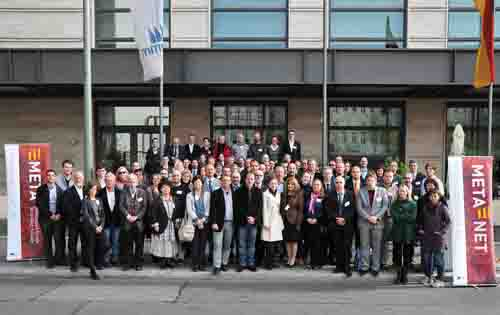
\includegraphics[width=\textwidth]{../_media/meta-net_team.jpg}
  \caption{Etwa 100 Experten des Gebiets Sprachtechnologie -- Repräsentanten der in META-NET vertretenen Länder und Sprachen -- diskutierten und finalisierten die zentralen Ergebnisse der Weißbuch-Serie bei einem META-NET-Treffen in Berlin am 21./22.~Oktober 2011.}
\end{figure}

\end{document}

